 % The main file for CAMP reports
 % Don't put any content in here. 
 % Don't even include content files by using \input or \inlcude. 
 % Put your content to TEXT.TEX or include it there using \input.
 % Uses:
 %		SETTINGS.TEX	contains the settings for this document
 %		COMMANDS.TEX	contains commands which can be used while writing
 %		INFO.TEX			contains the author, title and so on for the cover
 %		COVER.TEX			formats the front cover of the document
 %		ABSTRACT.TEX	contains the abstract to be included (if needed)
 %		TEXT.TEX			contains the actual content of the document
 %		BIB.BIB				containt the BibTeX entries for the document


%% Draft document mode
%% Final document
\documentclass[11pt,a4paper,bibtotoc,idxtotoc,headsepline,footsepline,footexclude,BCOR12mm,DIV13]{scrbook}

%\documentclass[11pt,a4paper,bibtotoc,idxtotoc,headsepline,footsepline,footexclude,BCOR20mm,DIV10]{scrbook}

% KOMA-Optionen:
%  bibtotoc: include bibliography in table of contents
%  idxtotoc: include index in table of contents
%  headsepline: use horizontalline under heading
%  BCOR: binding correcion (Bindungskorrektur) (e.g.: BCOR5mm)
%  DIV: Number of sheet sections (used for layout) (e.g.: DIV12) 



% include title and author information for the cover
% Set here the title, authors and other stuff to be used for the cover
% This file is used by MAIN.TEX

% set title, authors and stuff for the cover
\def\doctype{Masterarbeit in Informatik}
\def\title{Runtime Protection against Advanced Code Reuse Attacks by Static Instrumentation of Binaries}
\def\titleGer{Laufzeitschutz gegen fortgeschrittene Code Wiederverwendungs-Angriffe durch statische Instrumentierung von Bin{\"a}rdateien}
\def\author{Matthias Konstantin Fischer}
\def\date{November 7th, 2016}

% text to appear in the footer
\def\footertext{}

% include settings
% Included by MAIN.TEX
% Defines the settings for the CAMP report document

\renewcommand{\sectfont}{\normalfont \bfseries}        % Schriftart der Kopfzeile

% manipulate footer
\usepackage{scrpage2}
\pagestyle{scrheadings}
\ifoot[\footertext]{\footertext} % \footertext set in INFO.TEX
%\setkomafont{pagehead}{\normalfont\rmfamily}
\setkomafont{pagenumber}{\normalfont\rmfamily}

%% allow sophisticated control structures
\usepackage{ifthen}

% use Palatino as default font
\usepackage{palatino}

% enable special PostScript fonts
\usepackage{pifont}

% make thumbnails
\usepackage{thumbpdf}

%to use the subfigures
\usepackage{subfigure}


\usepackage{colortbl}


%% show program code\ldots
%\usepackage{verbatim}
%\usepackage{program}

%% enable TUM symbols on title page
\usepackage{styles/tumlogo}


\usepackage{multirow}

%% use colors
\usepackage{color}

%% make fancy math
\usepackage{amsmath}
\usepackage{amsfonts}
\usepackage{amssymb}
\usepackage{textcomp}
\usepackage{yhmath} % f�r die adots 
%% mark text as preliminary
%\usepackage[draft,german,scrtime]{prelim2e}

%% create an index
\usepackage{makeidx}

% for the program environment
\usepackage{float}

%% load german babel package for german abstract
%\usepackage[german,american]{babel}
\usepackage[german,english, croatian]{babel}
\selectlanguage{english}
% use german characters as well
\usepackage[latin1, utf8]{inputenc}       % allow Latin1 characters

% use initals dropped caps - doesn't work with PDF
%\usepackage{dropping}


\usepackage{styles/shortoverview}
%----------------------------------------------------
%      Graphics and Hyperlinks
%----------------------------------------------------

%% check for pdfTeX
\ifx\pdftexversion\undefined
 %% use PostScript graphics
 \usepackage[dvips]{graphicx}
 \DeclareGraphicsExtensions{.eps,.epsi}
 \graphicspath{{figures/}{figures/review}} 
 %% allow rotations
 \usepackage{rotating}
 %% mark pages as draft copies
 %\usepackage[english,all,light]{draftcopy}
 %% use hypertex version of hyperref
 \usepackage[hypertex,hyperindex=false,colorlinks=false]{hyperref}
\else %% reduce output size \pdfcompresslevel=9
 %% declare pdfinfo
 %\pdfinfo { 
 %  /Title (my title) 
 %  /Creator (pdfLaTeX) 
 %  /Author (my name) 
 %  /Subject (my subject	) 
 %  /Keywords (my keywords)
 %}
 %% use pdf or jpg graphics
 \usepackage[pdftex]{graphicx}
 \DeclareGraphicsExtensions{.jpg,.JPG,.png,.pdf,.eps}
 \graphicspath{{figures/}} 
 
 %% Load float package, for enabling floating extensions
 \usepackage{float}
 
 %% allow rotations
 \usepackage{rotating}
 %% use pdftex version of hyperref
 \usepackage[pdftex,colorlinks=true,linkcolor=red,citecolor=red,%
 anchorcolor=red,urlcolor=red,bookmarks=true,%
 bookmarksopen=true,bookmarksopenlevel=0,plainpages=false%
 bookmarksnumbered=true,hyperindex=false,pdfstartview=%
 ]{hyperref}
%
%\usepackage[pdftex,colorlinks=false,linkcolor=red,citecolor=red,%
% anchorcolor=red,urlcolor=red,bookmarks=true,%
% bookmarksopen=true,bookmarksopenlevel=0,plainpages=false%
% bookmarksnumbered=true,hyperindex=false,pdfstartview=%
% ]{hyperref}
\fi




%% Fancy chapters
%\usepackage[Lenny]{fncychap}
%\usepackage[Glenn]{fncychap}
%\usepackage[Bjarne]{fncychap}

%\usepackage[avantgarde]{quotchap}

% set the bibliography style
%\bibliographystyle{styles/bauermaNum}
%\bibliographystyle{alpha}
\bibliographystyle{plain}

% include commands
% Commands to be used within the TUM report document
% Included by MAIN.TEX
% Please include your own cool commands here. 
% Be only sure to comment it sufficiently so others can use it.

%-------------------------------------------------------------
%                      Own Commands
%-------------------------------------------------------------


%-------------------------------------------------------------
% math stuff -------------------------------------------------

% nice R, N, C
\newcommand{\nat}{\mathbb{N}}
\newcommand{\real}{\mathbb{R}}
\newcommand{\compl}{\mathbb{C}}



% norm
\newcommand{\norm}[1]{\left\| #1 \right\|}

% un demi
\newcommand{\half}{\frac{1}{2}}

% parantheses
\newcommand{\parenth}[1]{ \left( #1 \right) }
\newcommand{\bracket}[1]{ \left[ #1 \right] }
\newcommand{\accolade}[1]{ \left\{ #1 \right\} }
%\newcommand{\angle}[1]{ \left\langle  #1 \right\rangle }

% partial derivative: %#1 function, #2 which variable
% simple / single line version
\newcommand{\pardevS}[2]{ \delta_{#1} f(#2) }
% fraction version
\newcommand{\pardevF}[2]{ \frac{\partial #1}{\partial #2} }

% render vectors: 3 and 4 dimensional
\newcommand{\veciii}[3]{\left[ \begin{array}[h]{c} #1 \\ #2 \\ #3	\end{array} \right]}
\newcommand{\veciv}[4]{\left[ \begin{array}[h]{c} #1 \\ #2 \\ #3 \\ #4	\end{array} \right]}

% render matrices: 3  dimensional (arguments in row first order)
\newcommand{\matiii}[9]{\left[ \begin{array}[h]{ccc} #1 & #2 & #3 \\ #4 & #5 & #6 \\ #7 & #8 & #9	\end{array} \right]}
%DOESN'T WORK,DON'T KNOW WHY \newcommand{\mativ}[16]{\left[ \begin{array}[h]{cccc} #1 & #2 & #3 & #4 \\ #5 & #6 & #7 & #8 \\ #9 & #10 & #11 & #12 \\ #13 & #14 & #15 & #16 \end{array} \right]}


%-------------------------------------------------------------
%-------------------------------------------------------------


%-------------------------------------------------------------
% some abreviations ------------------------------------------
\newcommand{\Reg}{$^{\textregistered}$}
\newcommand{\reg}{$^{\textregistered}$ }
\newcommand{\Tm}{\texttrademark}
\newcommand{\tm}{\texttrademark~}
\newcommand {\bsl} {$\backslash$}

%-------------------------------------------------------------
%-------------------------------------------------------------


%-------------------------------------------------------------
% formating --------------------------------------------------

% Theorem & Co environments and counters
\newtheorem{theorem}{Theorem}[chapter]
\newtheorem{lemma}[theorem]{Lemma}
\newtheorem{corollary}[theorem]{Corollary}
\newtheorem{remark}[theorem]{Remark}
\newtheorem{definition}[theorem]{Definition}
\newtheorem{equat}[theorem]{Equation}
\newtheorem{example}[theorem]{Example}
\newtheorem{algorithm_theo}[theorem]{Algorithm}

% inserting figures
\newcommand{\insertfigure}[4]{ % Filename, Caption, Label, Width percent of textwidth
	\begin{figure}[htbp]
		\begin{center}
			\includegraphics[width=#4\textwidth]{#1}
		\end{center}
		\vspace{-0.4cm}
		\caption{#2}
		\label{#3}
	\end{figure}
}




% referecing figures

\newcommand{\refFigure}[1]{ %label
	figure \ref{#1}
}
\newcommand{\refChapter}[1]{ %label
	chapter \ref{#1}
}

\newcommand{\refSection}[1]{ %label
	section \ref{#1}
}

\newcommand{\refParagraph}[1]{ %label
	paragraph \ref{#1}
}

\newcommand{\refEquation}[1]{ %label
	equation \ref{#1}
}

\newcommand{\refTable}[1]{ %label
	table \ref{#1}
}


% \newcommand{\todo}[1]{#1}


\newcommand{\rigidTransform}[2]
{
	${}^{#2}\!\mathbf{H}_{#1}$
}

%code, in typewriter
\newcommand{\code}[1]
 {\texttt{#1}}

% comment that appears on the border - very practical !!!
\newcommand{\comment}[1]{\marginpar{\raggedright \noindent \footnotesize {\sl #1} }}

% page clearing
\newcommand{\clearemptydoublepage}{%
  \ifthenelse{\boolean{@twoside}}{\newpage{\pagestyle{empty}\cleardoublepage}}%
  {\clearpage}}


%-------------------------------------------------------------
%-------------------------------------------------------------


\newcommand{\etAl}{\emph{et al.}\mbox{ }}


%\makeindex
	%% inter line spacing
%\linespread{1.0}

\makeglossary

\begin{document}

	\frontmatter
	
	
	% The front cover for the TUM report document.
% Included by MAIN.TEX


%--------------------------------------------------
% The Front Cover
%--------------------------------------------------

% The front cover for the TUM document.
% Included by MAIN.TEX


%--------------------------------------------------
% The Front Cover
%--------------------------------------------------

% correct BCOR - undo at the end !!!
\def\bcorcor{0.15cm}
\addtolength{\hoffset}{\bcorcor}

\thispagestyle{empty}

 \vspace{4cm}
\begin{center}
	       \oTUM{4cm}
	   
	   \vspace{5mm}     
	   \huge FAKULT{\"A}T F{\"U}R INFORMATIK\\ 
	   \vspace{0.5cm}
	 \large DER TECHNISCHEN UNIVERSIT{\"A}T M{\"U}NCHEN\\
    \vspace{1mm}
        
	\end{center}
		

\vspace{15mm}
\begin{center}

   {\Large \doctype}

  \vspace{20mm}
  
  {\huge\bf \title}\\%[3ex]
  
  
  \vspace{15mm}
  
  
  {\LARGE  \author}
  
  \vspace{5mm}
  
  \begin{figure}[h!]
  \centering
   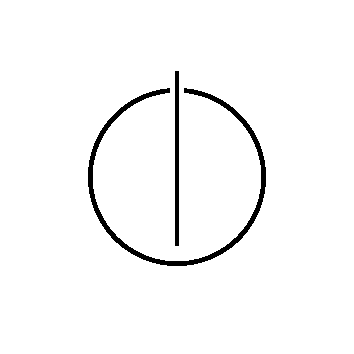
\includegraphics[width=4cm]{styles/informat.png}
  \end{figure}
  
  \end{center}
%	\clearemptydoublepage
%	
%	% The titlepage for the CAMP report document.
% Included by MAIN.TEX


%--------------------------------------------------
% The title page
%--------------------------------------------------

% correct BCOR - undo at the end !!!
\def\bcorcor{0.15cm}
\addtolength{\hoffset}{\bcorcor}

\thispagestyle{empty}

 \vspace{10mm}
\begin{center}
	       \oTUM{4cm}
	   
	   \vspace{5mm}     
	   \huge FAKULT{\"A}T F{\"U}R INFORMATIK\\ 
	   \vspace{0.5cm}
	 \large DER TECHNISCHEN UNIVERSIT{\"A}T M{\"U}NCHEN\\
        
	\end{center}
		

\vspace{5mm}
\begin{center}

   {\Large \doctype}

  \vspace{5mm}
  
  {\LARGE \title}\\
  
  
  \vspace{5mm}
  
  
  {\LARGE  \titleGer}\\
  
  
  \vspace{5mm}

    %\hfill
    \begin{tabular}{ll}
	   \Large Author:        & \Large \author \\[2mm]
	   \Large Supervisor:    & \Large Prof. Dr. Claudia Eckert \\[2mm]				
	   \Large Advisor:	 & \Large M.Sc. Paul Muntean \\[2mm]
	   \Large Date:          & \Large November 7th, 2016
	 \end{tabular}
	 
	 
	 \begin{figure}[h!]
  \centering
   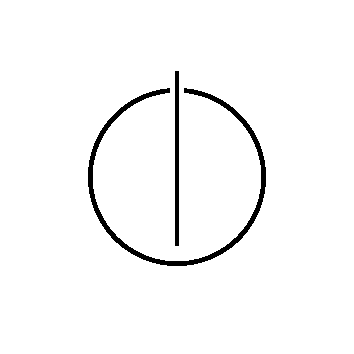
\includegraphics[width=4cm]{styles/informat.png}
  \end{figure}
   

\end{center}

% undo BCOR correction
\addtolength{\hoffset}{\bcorcor}
	
	
%	\input{components/cover_maschmeyer}
	\clearemptydoublepage
	
	% The titlepage for the CAMP report document.
% Included by MAIN.TEX


%--------------------------------------------------
% The title page
%--------------------------------------------------

% correct BCOR - undo at the end !!!
\def\bcorcor{0.15cm}
\addtolength{\hoffset}{\bcorcor}

\thispagestyle{empty}

 \vspace{10mm}
\begin{center}
	       \oTUM{4cm}
	   
	   \vspace{5mm}     
	   \huge FAKULT{\"A}T F{\"U}R INFORMATIK\\ 
	   \vspace{0.5cm}
	 \large DER TECHNISCHEN UNIVERSIT{\"A}T M{\"U}NCHEN\\
        
	\end{center}
		

\vspace{5mm}
\begin{center}

   {\Large \doctype}

  \vspace{5mm}
  
  {\LARGE \title}\\
  
  
  \vspace{5mm}
  
  
  {\LARGE  \titleGer}\\
  
  
  \vspace{5mm}

    %\hfill
    \begin{tabular}{ll}
	   \Large Author:        & \Large \author \\[2mm]
	   \Large Supervisor:    & \Large Prof. Dr. Claudia Eckert \\[2mm]				
	   \Large Advisor:	 & \Large M.Sc. Paul Muntean \\[2mm]
	   \Large Date:          & \Large November 7th, 2016
	 \end{tabular}
	 
	 
	 \begin{figure}[h!]
  \centering
   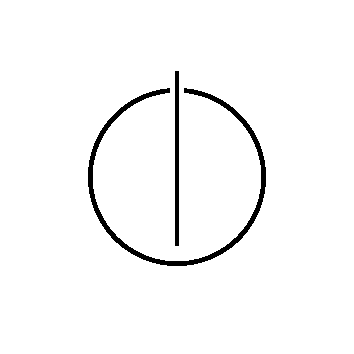
\includegraphics[width=4cm]{styles/informat.png}
  \end{figure}
   

\end{center}

% undo BCOR correction
\addtolength{\hoffset}{\bcorcor}
	
	
	\clearemptydoublepage


\thispagestyle{empty}
\selectlanguage{german}
	\vspace*{0.8\textheight}
	\noindent
	I confirm that this master’s thesis in informatics is my own work and I have documented
        all sources and material used.
	
	\vspace{15mm}
	\noindent
	M{\"u}nchen, den \today \hspace{5cm} \author
\selectlanguage{english}
\newpage
	
	\clearemptydoublepage
\phantomsection
\addcontentsline{toc}{chapter}{Acknowledgements}	


%\chapter*{Acknowledgements}

\vspace*{2cm}

\begin{center}
{\Large \bf Acknowledgments}
\end{center}

\vspace{1cm}




If someone contributed to the thesis... might be good to thank them here.
	
	
%MA Thesis
% Applications like firefox, chrome, mysql, postgresql or nginx are written in C/C++ 
% mostly for performance reasons or to have better control thereover, availability 
% and a vast number of third party libraries are other strong reasons. Yet using 
% these languages comes at the price of allowing code reusage attacks, as up to this
% day buffer overflows and other memory corruption exploits are haunting the various
% projects using C/C++. This is not the main focus, but only a prerequisite of the 
% attacks we are going to discuss. The language c++, which initially was built based
% on C introduced the concept of inheritance to allow for more flexible designs. 
% This modelled by storing a pointer to a table that stores the virtual functions 
% of the particular object. The relatively recently discovered COOP exploits and its
% successors leverage this pointer to change the control flow hijacking the attacked
% program. Although C does not employ the concept of virtual calls, it is still 
% attackable by modifying global code pointers as shown in the Control Flow Bending
% paper.
% 
% While there exists extensive work to protect binaries from the source level, 
% one might not have access to the the sourcecode or compilation process, 
% therefore binary based solutions must also be considered , of which there
% are near to none that can mitigate COOP exploits. In this thesis, we present
% \textsc{TypeShield} a tool implemented ontop of the principles introduced by
% TypeArmor, which reportedly can mitiagte COOP attacks to a certain extent. 
% We partially verify the results of TypeArmor and implement our own matching
% schema based on the parameter wideness of callsites and calltargets. 
% Our classification schema achieves an additional reduction of the possible
% calltargets per callsite of up to 20\% with an overall reduction of about 
% 9\% when comparing to parameter count based aproaches.



%Paper abstract
High security, high performance and high availability 
applications such as the Firefox and Chrome web browsers 
are implemented in C/C++ for modularity, performance and 
compatibility to name just a few reasons.
Virtual functions, which facilitate late binding,
are a key ingredient in facilitating run-time polymorphism
in C++ because it allows and object to use general (its own) 
or specific functions (inherited) contained in the class hierarchy.
However, because of the specific implementation of late binding,
which performs no verification in order to check where an indirect call site 
(virtual object dispatch through virtual pointers (\textit{vptrs})) is allow to
call inside the class hierarchy, this opens a large attack surface which
was successfully exploited by the COOP attack.
Since manipulation (changing or inserting new \textit{vptrs}) violates the 
programmer initial pointer semantics and allows an attacker to
redirect the control flow of the program as he desires, \textit{vptrs} corruption
has serious security consequences similar to those of other 
data-only corruption vulnerabilities.
Despite the alarmingly high number of \textit{vptr} corruption
vulnerabilities, the \textit{vptr} corruption problem has not
been sufficiently addressed by the researchers.

In this paper, we present \textit{TypeShild}, a run-time \textit{vptr} corruption
detection tool. It is based on executable instrumentation at load time
and uses a novel run-time type and function parameter counter technique
in order to overcome the limitations of current approaches and efficiently
verify dynamic dispatching during run-time.
In particular, \textit{TypeShild} can be automatically and easily used
in conjunction with legacy applications or where source code is missing.
It achieves higher caller/caller matching (precision) and with reasonable
run-time overhead.
We have applied \textit{TypeShild} to real life software such as
web servers, JavaScript engines, FTP servers and large-scale software
including Chrome and Firefox browsers, and were able to efficiently
and with low performance overhead to protect this applications from 
\textit{vptr} corruptions vulnerabilities.
Our evaluation shows that our target reduction schema achieves an additional
reduction of the possible call targets per call-site of up to 
20\% with an overall reduction of about 9\% when comparing to other
parameter count based approaches.


	\tableofcontents
  
  \clearemptydoublepage

\phantomsection
\addcontentsline{toc}{chapter}{Outline of the Thesis}

\begin{center}
	\huge{Outline of the Thesis}
\end{center}




%--------------------------------------------------------------------
\section*{Part I: Introduction and Theory}

\noindent {\scshape Chapter 1: Introduction}  \vspace{1mm}

\noindent  This chapter presents an overview of the thesis and it purpose. Furthermore, it will discuss the sense of life in a very general approach.  \\

\noindent {\scshape Chapter 2: Theory}  \vspace{1mm}

\noindent  No thesis without theory.   \\

%--------------------------------------------------------------------
\section*{Part II: The Real Work}

\noindent {\scshape Chapter 3: Overview}  \vspace{1mm}

\noindent  This chapter presents the requirements for the process.

	\mainmatter
	
	
		% ---------------------------------------------------------------------------
		%
		%Introduction and Background Theory
		%
		% ---------------------------------------------------------------------------
		%\part[Introduction and Theory]{Introduction and Theory}
		%\label{part:introAndBackgroundTheory}
		\section{Introduction}
\label{chapter:Introduction}
In this Chapter we present the motivation of our work in Section~\ref{Motivation}.
Section~\ref{Contribution} presents the contribution of our work.
Finally, Section~\ref{Outline} depicts the thesis outline.

\textbf{Motivation.}
\label{Motivation}
Control-Flow Integrity (CFI)~\cite{abadi:cfi2, abadi:cfi} is one of the most used techniques to secure program execution flows against advanced Code-Reuse Attacks (CRAs).
Advanced CRAs such as the recently published COOP~\cite{schuster:coop} and its extensions \cite{crane:readactor++} or the attacks described by the Control Flow Bending paper \cite{carlini:bending} are able to bypass most traditional CFI solutions, as they focus on indirect callsites, which are not as easy to decide at compile time.

This is a problem for applications written in C++, as one of its principle is inheritance and virtual functions. The concept of virtual functions allows the programmer to overwrite a virtual function of the baseclass with his own implementation. While this allows for much more flexible code, this flexibility is the reason COOP actually works. The problem is that in order to implement virtual functions, the compiler needs to generate a table of all virtual functions for each class containing them and provide each instanciation of such a class with a pointer to said table. COOP now leverages a memory corruption to inject their own object with a fake virtual pointer, which basically gives him control over the whole program, while the control flow still looks genuine, as no code was replaced. 

There exist several source code based solutions that either insert runtime checks during the compilation of the program like SafeDispatch \cite{safedispatch:jang}, ShrinkWrap \cite{haller:shrinkwrap} or IFCC/VTV \cite{vtv:tice}, which is the solution it is based on. Others modify and reorder the contents of the virtual table as their main aspect like the paper by Bounov et al \cite{bounov:interleaving}. While the recently published redactor++ \cite{crane:readactor++} implements a combination of those ideas.

While this might seem that only C++ is vulnerable, while C is safe, this notion is wrong, as the Control Flow Bending paper \cite{carlini:bending} proposes attacks on nginx leveraging global function pointers, which are used to provide configurable behaviour.

As previously mentioned, there exist many solutions when one tries to tackle this problem while access to the application in question is provided. However, when we are faced with proprietary third party binaries, which are provided as is and without the actual sourcecode, the number of tools that can protect against COOP or similar attacks is rather low.

TypeArmor~\cite{veen:typearmor} is such a tool that implements a fine grained forward edge CFI solution for binaries. It calculates invariants for calltargets and indirect callsites based on the number of parameters they use by leveraging static analysis of the binary, which then is patched to enforce those invariants during runtime. However, as of today we are not able to access the source code of TypeArmor, which is why we implement our own approximation of the tool.

The main shortcoming of TypeArmor is that even with high precision in the classification of calltargets and callsites, one cannot exclude calltargets with lower parameter number from callsites, for one due compatability and also due to variadic functions, which are a special case in themselves. This basically means that when a callsite prepares 6 parameters, it is able to call all address taken functions.


We implemented \textit{TypeShield} to show a possible remedy of this problem by introducing parameter types into the classification of callsites and calltargets. 

\textbf{Contribution.}
\label{Contribution}
The goals of our thesis are twofold. First we attempt to verify the results as provided by the TypeArmor paper. Second, implement our own classification schema to fix some of the shortcomings of previous binary based approaches to further mitigate advanced code reuse attacks.

Our main contribution is thus the design and implementation of callsite and calltarget classification schema that is based on the wideness of parameters alone. We implemented configurable reaching and liveness analysis algorithms that operate on the full set of general purpose integer registers of a x86-64 CPU and evaluated various path merge operators. Although the basic idea of our aproach to rely only on the wideness of a type is rather simple, we still achieved a reduction of up to 20\% less callsites per calltarget with an overall of about 9\% when compared to our implementation of a parameter count based matching schema.


Furthermore, we implemented an approximation of the matching schema employed by TypeArmor proposed by \cite{veen:typearmor}, because we had no access to their sourcecode and could achieve similar results regarding parameter matching, partially verifying their results.

\textbf{Outline.}
\label{Outline}
The remainder of this thesis is organized as follows.
Chapter~\ref{chapter:TypeShild Overview} contains a high level overview of \textit{TypeShield}.
Chapter~\ref{chapter:Design} describes the theory used and decisions made during the design of \textit{TypeShield}.
Chapter~\ref{chapter:Implementation} briefly presents the implementation details of our tool.
Our \textit{TypeShield} implementation is evaluated and discussed in
Chapter~\ref{chapter:Evaluation} and Chapter~\ref{chapter:Discussion}, respectively.
Chapter~\ref{chapter:Related_Work} surveys related work.
Finally, Chapter~\ref{chapter:Future_Work} highlights several future venues of research while
Chapter~\ref{chapter:Conclusion} concludes this thesis.



		\chapter{Motivation}
\label{chapter:Introduction}


bla

		\chapter{Overview}
\label{chapter:Overview}

\section{Types Inference/Recovery from Binaries}
\subsection{Types Recovery in General}
\subsection{Function Parameter Types Recovery}
\subsection{Caller/Callee Parameter Types Recovery}

\section{Code-Reuse Attacks}
this section will up to 1 DIN A page. First talk about code reuse attacks in general and then 
about COOP.

Say why COOP is not affected by the following mittigation approaches
Talk about intel CET, talk about Windows CF guard.


\section{Control-Flow Integrity}

\section{Cntrol-Flow Integrity}
		\section{Evaluation}
\label{chapter:Evaluation}
We evaluated \textsc{TypeShield} by instrumenting various open source applications and analyzing the results. 
We used the two ftp server applications \textit{vsftpd} (v.1.1.0) and \textit{proftpd} (v.1.3.3), the two http server 
applications \textit{postgresql} (v.9.0.10) and \textit{mysql} (v.5.1.65), the memory cache application \textit{memcached} (v.1.4.20) 
and the \textit{node.js} server application (v.0.12.5). We chose these applications, which are a subset of the 
applications also used by the TypeAmor~\cite{veen:typearmor} to allow for later comparison.
In our evaluation we addressed the following research questions:
\begin{itemize}
 \item \textbf{RQ1:} How precise is \textsc{TypeShield}? (\cref{section:typeshieldprecision})

 \item \textbf{RQ2:} What level of security does \textsc{TypeShield} offer? (\cref{section:typeshieldeffectiveness})

 \item \textbf{RQ3:} What is the runtime overhead of \textsc{TypeShield}? (\cref{section:typeshieldoverheadperformance})

 \item \textbf{RQ4:} What is the instrumentation overhead of \textsc{TypeShield}? (\cref{section:typeshieldoverheadinstrumentation})

 \item \textbf{RQ5:} Is our tool better than other tools? (\cref{RQ5: Is TypeShield better than other tools?})
\end{itemize}
\textbf{Comparison Method.} As we do not have access (we requested the Authors several times to provide access to the source code) to the source code of TypeAmor, we implemented two modes in \textsc{TypeShield}. 
The first mode of our tool is an similar implementation of the \textit{count} 
policy described by TypeArmor. The second mode is our implementation of the \textit{type} policy on
top of our \textit{count} policy implementation. 
%
%\textbf{Experimental Setup.} We setup our environment within a VirtualBox (version 5.0.26r) instance, which runs Kubuntu 16.04 LTS (Linux Kernel
%version 4.4.0) and has access to 3GB of RAM and 4 of 8 provided hardware threads (Intel i7-4170HQ @ 2.50 GHz).

\subsection{RQ1: Precision of \textsc{TypeShield}}
\label{section:typeshieldprecision}
\todo[inline]{In this section we need just one or two Table similar to what TypeArmor contains, first we need to define the fields which make most sense.}

To measure the precision of \textsc{TypeShield}, we need to compare the classification of call-sites and call-targets as is given by our tool to
some sort of ground truth for our test targets. We generate this ground truth by compiling our test targets using a custom compiled Clang/LLVM
compiler (v.4.0.0 trunk 283889) with a MachineFunction pass inside the x86 code generation implementation of LLVM. We essentially 
collect three data points for each call-site/call-target from our LLVM-pass:
\textit{1)} The point of origination, which is either the name of the call-target or the name of the function the call-site resides in.
\textit{2)} The return type that is either expected by the call-site or provided by the call-target.
\textit{3)} The parameter list that is provided by the call-site or expected by the call-target, which discards the variadic argument list.

However, before we can proceed to measure the quality and precision of \textsc{TypeShield}'s classification of call-targets and call-sites
using our ground truth, we need to evaluate the quality and applicability of the ground truth, we collected.

\subsubsection{Quality and Applicability of Ground Truth}
\label{subsection:typeshieldprecision}
To assess the applicability of our collected ground truth, we essentially need to assess the structural compatibility of our two datasets.
First, we take a look at the comparability of call-targets and second, we take a look at the compatibility of call-sites. The results are depcited in Table \ref{tbl:matchingquality}.

\begin{table}[h!]
\resizebox{\columnwidth}{!}{
	\begin{tabular}{l|r|r|r|r|r|r}%
	\toprule
	\multicolumn{1}{c}{\bfseries O2} & \multicolumn{3}{c|}{ {\bfseries call-targets}} & \multicolumn{3}{c}{{\bfseries call-sites} }\\
	\bfseries Target & match & Clang miss &  tool miss &  match & Clang miss & tool miss% specify table head
	\\\midrule
	\csvreader[before filter=\ifthenelse{\equal{\csvcoli}{geomean}}{\csvfilterreject}{\csvfilteraccept},  late after line=\\, late after last line=\\\midrule]{csvs/matching.O2.csv}{
		%1=\target, 2=\opt, 3=\fns, 4=\fnsnotClang, 5=\fnsnotpadyn, 6=\ats, 7=\atnotClang, 8=\atnotpadyn, 9=\cscount, 10=\csClang, 11=\cspadyn
	}
	{\csvcoli & \csvcoliii & \csvcoliv (\csvcolv \% )& \csvcolvi (\csvcolvii \% )& \csvcolxiii & \csvcolxiv  (\csvcolxv) & \csvcolxvi   (\csvcolvii) }% specify your coloumns here

	\csvreader[before filter=\ifthenelse{\equal{\csvcoli}{geomean}}{\csvfilteraccept}{\csvfilterreject},  late after line=\\, late after last line=\\\bottomrule]{csvs/matching.O2.csv}{
		%1=\target, 2=\opt, 3=\fns, 4=\fnsnotClang, 5=\fnsnotpadyn, 6=\ats, 7=\atnotClang, 8=\atnotpadyn, 9=\cscount, 10=\csClang, 11=\cspadyn
	}
	{\csvcoli & \csvcoliii & \csvcoliv \ (\csvcolv \% )& \csvcolvi \ (\csvcolvii \% )& \csvcolxiii & \csvcolxiv \ (\csvcolxv) & \csvcolxvi \ (\csvcolvii) }% specify your coloumns here
    	\end{tabular}
    	
    	}
%     	}
	\caption {Table shows the quality of structural matching provided by our automated verify and test environment, 
	regarding call-sites and call-targets when compiling with optimization level O2. The label Clang miss 
	denotes elements not found in the data-set of the Clang/LLVM pass. The label tool miss denotes elements not found in the data-set of \textsc{TypeShield}.}
	\label{tbl:matchingquality}
\end{table}

\textbf{Call-targets.} The obvious choice for structural comparison regarding call-targets is their name, as these are simply functions. 
First, we have to remove internal functions from our data-sets like the \texttt{\_init} or \texttt{\_fini} functions, which are of no consequence for us. 
Furthermore, while C functions can simply be matched by their name as they are unique through the binary, the same cannot be said about the 
language C++. One of the key differences between C and C++ is function overloading, which allows to define several functions with the same name, as 
long as they differ in namespace or parameter type. As LLVM does not know about either concept, the Clang compiler needs to generate unique names. 
The method used for unique name generation is called mangling and composes the actual name of the function, its the return type, its name-space and the 
types of its parameter list. We therefore need to reverse this process and then compare the fully typed names.
Table \ref{tbl:matchingquality} shows three data points regarding call-targets for the optimization level O2:
\textit{1)}  The number of comparable call-targets that are found in both datasets
\textit{2)}  Clang miss: The number of call-targets that are found by \textsc{TypeShield} but not by our Clang/LLVM pass
\textit{3)}  tool miss: The number of call-targets that are found by our Clang/LLVM pass but not by \textsc{TypeShield}

The problematic column is the Clang miss column, as these might indicate problems with \textsc{TypeShield}. These numbers are relatively low (below 1\%) with only node showing a significant higher value than the rest (around 1.6\%). The column labeled tool miss lists 
higher numbers, however these are of no real concern to us, as our ground truth pass possibly collects more data: All source files used during the 
compilation of our test-targets are incorporated into our ground truth. The compilation might generate more than one binary and therefore not 
necessary all source files are used for our test-target.

Considering this, we can safely state that our structural matching between ground truth and \textsc{TypeShield} regarding call-targets is nearly
perfect (above 98\%)\\


\textbf{Call-sites.} While our structural matching of call-targets is rather simple, the matter of matching callsites is more complex. Our tool can provide accurate addressing of call-sites within the binary. However, Clang/LLVM does not have such capabilities in its intermediate representation (IR). Furthermore the IR is not the final representation within the compiler, as the IR is transformed into a machine-based representation (MR), which is the again optimized. Although we can read information regarding paramters from the IR, it is not possible with the MR. Therefore we attach that data directly after the conversion from IR to MR and read that data at the end of the compilation. To not unneccessarily pollute our dataset, we only considered call-targets, which have been found in both datasets. 
The table \ref{tbl:matchingquality} shows three data points regarding call-sites for the optimization level O2:
\textit{1)} The number of comparable call-sites that are found in both datasets.
\textit{2)} Clang miss: The number of call-sites that are discarded from the dataset of \textsc{TypeShield}.
\textit{3)} tool miss: The number of call-sites that are discarded from the dataset of our Clang/LLVM pass.

Both columns (Clang miss and tool miss) show a relatively low number of problems (<0.5\%), therefore we can also safely state that our structural matching between ground truth and \textsc{TypeShield} regarding call-sites is also nearly perfect (above 99\%)

\subsubsection{Classification Precision (\textit{count})}
\label{subsection:typeshieldcountprecision}

We measured two data points per target, the number and ratio of perfect classifications and the number and ratio of problematic classifications, which in the case of calltargets refers to overestimations and in case of callsites refers to underestimations. The results are depicted in Table \ref{tbl:precisionCOUNT}.
\begin{table}[h!]
\resizebox{\columnwidth}{!}{
	\begin{tabular}{l|r|r|r|r|r|r}%

	\toprule
	\multicolumn{1}{c}{\bfseries O2} & \multicolumn{3}{c}{\bfseries Call-targets} & \multicolumn{3}{c}{\bfseries Call-sites}\\
	
	\bfseries Target & \#  &  perfect &  problem & \# & perfect &  problem % specify table head
	\\\midrule
	\csvreader[before filter=\ifthenelse{\equal{\csvcolii}{geomean}}{\csvfilterreject}{\csvfilteraccept}, late after line=\\, late after last line=\\\midrule]{csvs/classification_comp.sources_union_follow.O2.csv}{
		%1=opt,2=target,3=cs,4=cs args,5=perfect,6=cs args,7=problem,8 = cs non-void ,9=correct,10 = cs non-void, 11=problem,12 = ct, 13 = ct args, 14=perfect, 15 = ct args, 16=problem, 17 = ct void, 18=correct, 19=ct void, 20=problem
}
	{\csvcolii  &  \csvcolxii & \csvcolxiii \ (\csvcolxiv \%) & \csvcolxv \ (\csvcolxvi \%) & \csvcoliii & \csvcoliv \ (\csvcolv \%) & \csvcolvi \ (\csvcolvii\%)}% specify your coloumns here

	\csvreader[before filter=\ifthenelse{\equal{\csvcolii}{geomean}}{\csvfilteraccept}{\csvfilterreject}, late after line=\\, late after last line=\\\bottomrule]{csvs/classification_comp.sources_union_follow.O2.csv}{
		%1=opt,2=target,3=cs,4=cs args,5=perfect,6=cs args,7=problem,8 = cs non-void ,9=correct,10 = cs non-void, 11=problem,12 = ct, 13 = ct args, 14=perfect, 15 = ct args, 16=problem, 17 = ct void, 18=correct, 19=ct void, 20=problem
}
	{\csvcolii  &  \csvcolxii & \csvcolxiii \ (\csvcolxiv \%) & \csvcolxv \ (\csvcolxvi \%) & \csvcoliii & \csvcoliv \ (\csvcolv \%) & \csvcolvi \ (\csvcolvii\%)}% specify your coloumns here
    	\end{tabular}

}
		\caption {The results for analysis using the \textit{count} policy on the O2 optimization level.}
		\label{tbl:precisionCOUNT}
\end{table}~\\
\textbf{Experiment Setup (Call-targets).} Union combination operator with an $analyze$ function that follows into occurring direct calls.
\textbf{Results (Call-targets).} The problem rate is under 0.01\%, as there are only two testtargets, that exhibit a problematic classification. The rate of perfect classification is in general over 80\% with mysql as an exception (73.85\%) resulting in a geometric mean of 86.86\%.
\textbf{Experiment Setup (Call-sites)} Union combination operator with an $analyze$ function that does not follow into occurring direct calls while relying on a backward inter-procedural analysis.
\textbf{Results (Call-sites).} The problem rate is under 0.01\%, as there is only one testtarget, that exhibit a problematic classification. The rate of perfect classification is in general over 60\% with nginx (48.49\%) and node (56.34\%) as an exception resulting in a geometric mean of 71.97\%.


\subsubsection{Classification Precision (\textit{type})}
\label{subsection:typeshieldcountprecision}

We measured two data points per testtarget, the number and ratio of perfect classifications and the number and ratio of problematic classifications, which in the case of calltargets refers to overestimations and in case of callsites refers to underestimations. The results are depicted in Table \ref{tbl:precisionTYPE}.
\begin{table}[h!]
\resizebox{\columnwidth}{!}{
	\begin{tabular}{l|r|r|r|r|r|r}%

	\toprule
	\multicolumn{1}{c}{\bfseries O2} & \multicolumn{3}{c}{\bfseries Call-targets} & \multicolumn{3}{c}{\bfseries Call-sites}\\
	
	\bfseries Target & \#  &  perfect &  problem & \# & perfect &  problem % specify table head
	\\\midrule
	\csvreader[before filter=\ifthenelse{\equal{\csvcolii}{geomean}}{\csvfilterreject}{\csvfilteraccept},  late after line=\\, late after last line=\\\midrule]{csvs/classification_comp2.type_exp6.O2.csv}{
		%1=opt,2=target,3=cs,4=cs args,5=perfect,6=cs args,7=problem,8 = cs non-void ,9=correct,10 = cs non-void, 11=problem,12 = ct, 13 = ct args, 14=perfect, 15 = ct args, 16=problem, 17 = ct void, 18=correct, 19=ct void, 20=problem
}
	{\csvcolii  &  \csvcolxii & \csvcolxiii \ (\csvcolxiv \%) & \csvcolxv \ (\csvcolxvi \%) & \csvcoliii & \csvcoliv \ (\csvcolv \%) & \csvcolvi \ (\csvcolvii\%)}% specify your coloumns here

	\csvreader[before filter=\ifthenelse{\equal{\csvcolii}{geomean}}{\csvfilteraccept}{\csvfilterreject},  late after line=\\, late after last line=\\\bottomrule]{csvs/classification_comp2.type_exp6.O2.csv}{
		%1=opt,2=target,3=cs,4=cs args,5=perfect,6=cs args,7=problem,8 = cs non-void ,9=correct,10 = cs non-void, 11=problem,12 = ct, 13 = ct args, 14=perfect, 15 = ct args, 16=problem, 17 = ct void, 18=correct, 19=ct void, 20=problem
}
	{\csvcolii  &  \csvcolxii & \csvcolxiii \ (\csvcolxiv \%) & \csvcolxv \ (\csvcolxvi \%) & \csvcoliii & \csvcoliv \ (\csvcolv \%) & \csvcolvi \ (\csvcolvii\%)}% specify your coloumns here
    	\end{tabular}

}
		\caption {The results for analysis using the \textit{type} policy on the O2 optimization level.}
		\label{tbl:precisionTYPE}
\end{table}~\\
\textbf{Experiment Setup (Call-targets).} Union combination operator with an $analyze$ function that does follow into occurring direct calls  and a vertical merge that intersects all reads until the first write.
\textbf{Results (Call-targets).} For half of the set, the problem rate is under 1\% and for the other half it is not above 10\%, resulting in a geomean of 1.92\%. The rate of perfect classification is in general over 70\% with nginx (69.38\%) and mysql (63.16\%)  resulting in a geometric mean of 77.15\%.
\textbf{Experiment Setup (Call-sites).} Union combination operator with an $analyze$ function that does not follow into occurring direct calls while relying on a backward inter-procedural analysis.
\textbf{Results (Call-sites).} For two thirds of the set, the problem rate is under 2\% and for last third it is not above 10\%, resulting in a geomean of 1.38\%.  The rate of perfect classification is in general over 50\% with node (44.76\%) as an exception resulting in a geometric mean of 68.35\%.


%
%
%Efficiency
%
%
\subsection{RQ2: Security Level of \textsc{TypeShield}}
\label{section:typeshieldeffectiveness}
\todo[inline]{In this section we need just one or two Table similar to what TypeArmor contains, 
first we need to define the fields which make most sense.}

\begin{table*}[htbp!]
\begin{center}
 \resizebox{2\columnwidth}{!}{
	\begin{tabular}{l|r|rcl|r|rcl|r|rcl|r|rcl|r}%

	\toprule
	\multicolumn{1}{c}{\bfseries O2} & \multicolumn{1}{c}{\bfseries AT} & \multicolumn{4}{c}{\bfseries \textit{count}*} & \multicolumn{4}{c}{\bfseries \textit{count}} & \multicolumn{4}{c}{\bfseries \textit{type}*} & \multicolumn{4}{c}{\bfseries \textit{type}}\\
	
	\bfseries Target && \multicolumn{3}{c}{ limit (mean $\pm$ $\sigma$)} & median & \multicolumn{3}{c}{ limit (mean $\pm$ $\sigma$)} & median & \multicolumn{3}{c}{ limit (mean $\pm$ $\sigma$)} & median & \multicolumn{3}{c}{ limit (mean $\pm$ $\sigma$)} & median  % specify table head
	\\\midrule
	\csvreader[before filter=\ifthenelse{\equal{\csvcolii}{geomean}}{\csvfilterreject}{\csvfilteraccept},  late after line=\\, late after last line=\\\midrule]{csvs/policy_compare_at.O2.csv}{
	%1=opt,2=target,3=at,4=count safe avg,5=count safe sig,6=count safe median,7=count prec avg,8=count prec sig,9=count prec median,10=count* avg,11=count* sig,12=count* median,13=type safe avg,14=type safe sig,15=type safe median,16=type prec avg,17=type prec sig,18=type prec median,19=type* avg,20=type* sig,21=type* median
 }
	{\csvcolii  &  \csvcoliii & \csvcolx & $\pm$ & \csvcolxi & \csvcolxii & \csvcolvii & $\pm$ & \csvcolviii& \csvcolix& \csvcolxix & $\pm$ & \csvcolxx& \csvcolxxi & \csvcolxvi & $\pm$ & \csvcolxvii& \csvcolxviii }% specify your coloumns here

	\csvreader[before filter=\ifthenelse{\equal{\csvcolii}{geomean}}{\csvfilteraccept}{\csvfilterreject},  late after line=\\, late after last line=\\\bottomrule]{csvs/policy_compare_at.O2.csv}{
	%1=opt,2=target,3=at,4=count safe avg,5=count safe sig,6=count safe median,7=count prec avg,8=count prec sig,9=count prec median,10=count* avg,11=count* sig,12=count* median,13=type safe avg,14=type safe sig,15=type safe median,16=type prec avg,17=type prec sig,18=type prec median,19=type* avg,20=type* sig,21=type* median
 }
	{\csvcolii  &  \csvcoliii & \csvcolx & $\pm$ & \csvcolxi & \csvcolxii & \csvcolvii & $\pm$ & \csvcolviii& \csvcolix& \csvcolxix & $\pm$ & \csvcolxx& \csvcolxxi & \csvcolxvi & $\pm$ & \csvcolxvii& \csvcolxviii }% specify your coloumns here

    	\end{tabular}

}
	\caption {The results of comparing our implementation results with the theoretical limits for the different restriction policies combined with an address taken analysis for optimization level O2.}
	\label{tbl:policycompat}
\end{center}
\end{table*}

We are now going to evaluate the effectiveness of \textsc{TypeShield} leveraging the result of several experiment runs: First we are going to establish a baseline using the data 
collected from our Clang/LLVM pass, which are the theoretical limits our implementation can reach for both the \textit{count} and the \textit{type} schema. Second we are going to evaluate the effectiveness of our \textit{count} 
policy and third we are going to evaluate the effectiveness of our \textit{type} policy. For each series we collected three data points per test target, the average number of call-targets per call-site, the standard deviation $\sigma$ and the median. The results are depicted in table \ref{tbl:policycompat}. 

\subsubsection{Theoretical Limits.}
\label{subsection:theoreticallimit}
We explore the theoretical limits regarding the effectiveness of the \textit{count} and \textit{type} policies by relying on the collected ground truth data, essentially assuming perfect classification.
\textbf{Experiment Setup.} Based on the type information collected by our Clang/LLVM pass, we conducted two experiment series.
We derived the available number of call-targets for each call-site based on the collected ground truth applying the \textit{count} and \textit{type} schema

\textbf{Results.}
\textit{1)} The theoretical limit of the \textit{count*} schema has a geometric mean of 233 possible call-targets, which is 16.48\% of the geometric mean of total available 
call-targets, and
\textit{2)} The theoretical limit of the \textit{type*} schema has a geometric mean of 210 possible call-targets, which is 14.86\% of the geometric mean of total available
call-targets.

When compared, the theoretical limit of the \textit{type} policy allows about 10\% less available call-targets in the geomean in O2 than the limit of the \textit{count} policy.

\subsubsection{Reduction achieved by \textsc{TypeShield}}
\label{subsection:typeshieldvslimitcount}
\textbf{Experiment Setup.} We setup our two experiment series based on our previous evaluations regarding the classification precision for the \textit{count} and the \textit{type} policy.

\textbf{Results.}
\textit{1)}  The \textit{count} schema has a geometric mean of 315 possible call-targets, which is 22.29\% of the geometric mean of total available 
call-targets. This is 35.19\% more than the theoretical limit of available call-targets per call-site, and
\textit{2)}  The \textit{type} schema has a geometric mean of 290 possible call-targets, which is 20.52\% of the geometric mean of total available
call-targets. This is 38.09\% more than the theoretical limit of available call-targets per call-site.

When compared, our implementation of the \textit{type} policy allows about 7.93\% less available call-targets in the geomean in O2 than our implementation of the \textit{type} policy.


%\begin{table}[h!]
%\resizebox{.4\textwidth}{!}{
%	\begin{tabular}{l|c|rcl|c|rcl|c}%
%
%	\toprule
%	\multicolumn{1}{c}{\bfseries O2} & \multicolumn{1}{c}{\bfseries AT} & \multicolumn{4}{c}{\bfseries \textit{count} safe} & \multicolumn{4}{c}{\bfseries \textit{count} prec}\\
%	
%	\bfseries Target && \multicolumn{3}{c}{ limit (mean $\pm$ $\sigma$)} & median & \multicolumn{3}{c}{ limit (mean $\pm$ $\sigma$)} & median  % specify table head
%	\\\midrule
%	\csvreader[ late after line=\\, late after last line=\\\midrule]{../MA_Pictures/policy_compare_at.O2.csv}{
%	%1=opt,2=target,3=at,4=count safe avg,5=count safe sig,6=count safe median,7=count prec avg,8=count prec sig,9=count prec median,10=count* avg,11=count* sig,12=count* median,13=type safe avg,14=type safe sig,15=type safe median,16=type prec avg,17=type prec sig,18=type prec median,19=type* avg,20=type* sig,21=type* median
% }
%	{\csvcolii  &  \csvcoliii & \csvcoliv & $\pm$ & \csvcolv & \csvcolvi & \csvcolvii & $\pm$ & \csvcolviii& \csvcolix}% specify your coloumns here
%
%    	\end{tabular}
%}
%		\caption {The results of comparing \textit{count} safe and precision implementation restricted using an address taken analysis throughout different optimizations.}
%		\label{tbl:policycompatcount}
%\end{table}
%
%\begin{table}[h!]
%\resizebox{.4\textwidth}{!}{
%	\begin{tabular}{l|c|rcl|c|rcl|c}%
%
%	\toprule
%	\multicolumn{1}{c}{\bfseries O2} & \multicolumn{1}{c}{\bfseries AT} & \multicolumn{4}{c}{\bfseries \textit{type} safe} & \multicolumn{4}{c}{\bfseries \textit{type} prec}\\
%	
%	\bfseries Target && \multicolumn{3}{c}{ limit (mean $\pm$ $\sigma$)} & median & \multicolumn{3}{c}{ limit (mean $\pm$ $\sigma$)} & median  % specify table head
%	\\\midrule
%	\csvreader[ late after line=\\, late after last line=\\\midrule]{../MA_Pictures/policy_compare_at.O2.csv}{
%	%1=opt,2=target,3=at,4=count safe avg,5=count safe sig,6=count safe median,7=count prec avg,8=count prec sig,9=count prec median,10=count* avg,11=count* sig,12=count* median,13=type safe avg,14=type safe sig,15=type safe median,16=type prec avg,17=type prec sig,18=type prec median,19=type* avg,20=type* sig,21=type* median
% }
%	{\csvcolii  &  \csvcoliii & \csvcolxiii & $\pm$ & \csvcolxiv & \csvcolxv & \csvcolxvi & $\pm$ & \csvcolxvii& \csvcolxviii}% specify your coloumns here
%
%    	\end{tabular}
%}
%		\caption {The results of comparing \textit{type} safe and precision implementation restricted using an address taken analysis throughout different optimizations.}
%		\label{tbl:policycompattype}
%\end{table}

%
%\newpage
%\section{Security Analysis of \textsc{TypeShield}}
%\label{section:typeshieldsecurityanalysis}
%
%In this section, we discuss how effective \textsc{TypeShield} is 
%stopping advance code-reuse attacks (CRAs).
%Patching Policies
%Two types of diagrams. Table 5 from TypeArmor and a CDF to compare param count and param type. (baseline)
%here we put the CDF graphs from. There is no accurate security metrics to asses the security level of the enforced policy.
%
%
%
%\begin{table}
%\centering
%\resizebox{0.8\textwidth}{!}{
%	\begin{tabular}{l|c|c|c|c|c|c|c|c|c}%
%	\toprule
%	\multicolumn{1}{c}{\bfseries O0} & \multicolumn{1}{c}{} & \multicolumn{8}{|c}{ {\bfseries parameters}} \\
%	\bfseries Target & \bfseries \#CS & \bfseries -x & \bfseries +0 & \bfseries +1 & \bfseries +2 & \bfseries +3 & \bfseries +4 & \bfseries +5 & \bfseries +6 % specify table head
%	\\\midrule
%	\csvreader[ late after line=\\, late after last line=\\\midrule]{../MA_Pictures/classification_cs.O0.csv}{
%		%1=target,2=opt,3=cs,4=problems,5=+0,6=+1,7=+2,8=+3,9=+4,10=+5,11=+6,12=non-void-ok,13=non-void-problem
%	}
%	{\csvcoli & \csvcoliii & \csvcoliv & \csvcolv & \csvcolvi & \csvcolvii & \csvcolviii & \csvcolix & \csvcolx & \csvcolxi }% specify your coloumns here
%
%	\multicolumn{1}{c}{\bfseries O1}
%	\\\midrule
%	\csvreader[ late after line=\\, late after last line=\\\midrule]{../MA_Pictures/classification_cs.O1.csv}{
%		%1=target,2=opt,3=cs,4=problems,5=+0,6=+1,7=+2,8=+3,9=+4,10=+5,11=+6,12=non-void-ok,13=non-void-problem
%	}
%	{\csvcoli & \csvcoliii & \csvcoliv & \csvcolv & \csvcolvi & \csvcolvii & \csvcolviii & \csvcolix & \csvcolx & \csvcolxi}% specify your coloumns here
%
%	\multicolumn{1}{c}{\bfseries O2}
%	\\\midrule
%	\csvreader[ late after line=\\, late after last line=\\\midrule]{../MA_Pictures/classification_cs.O2.csv}{
%		%1=target,2=opt,3=cs,4=problems,5=+0,6=+1,7=+2,8=+3,9=+4,10=+5,11=+6,12=non-void-ok,13=non-void-problem
%	}
%	{\csvcoli & \csvcoliii & \csvcoliv & \csvcolv & \csvcolvi & \csvcolvii & \csvcolviii & \csvcolix & \csvcolx & \csvcolxi}% specify your coloumns here
%
%	\multicolumn{1}{c}{\bfseries O3}
%	\\\midrule
%	\csvreader[ late after line=\\, late after last line=\\\bottomrule]{../MA_Pictures/classification_cs.O3.csv}{
%		%1=target,2=opt,3=cs,4=problems,5=+0,6=+1,7=+2,8=+3,9=+4,10=+5,11=+6,12=non-void-ok,13=non-void-problem
%	}
%	{\csvcoli & \csvcoliii & \csvcoliv & \csvcolv & \csvcolvi & \csvcolvii & \csvcolviii & \csvcolix & \csvcolx & \csvcolxi}% specify your coloumns here
%
%
%    	\end{tabular}
%	}
%		\caption {Table shows the overestimation of the parameter count in matched callsites occurring in our precision focussed implementation of the \textit{count} policy, with -x denoting problematic callsites, when compiling with optimization levels O0 through O3}
%	\label{tbl:baselinecs}
%\end{table}
%
%\begin{figure}
%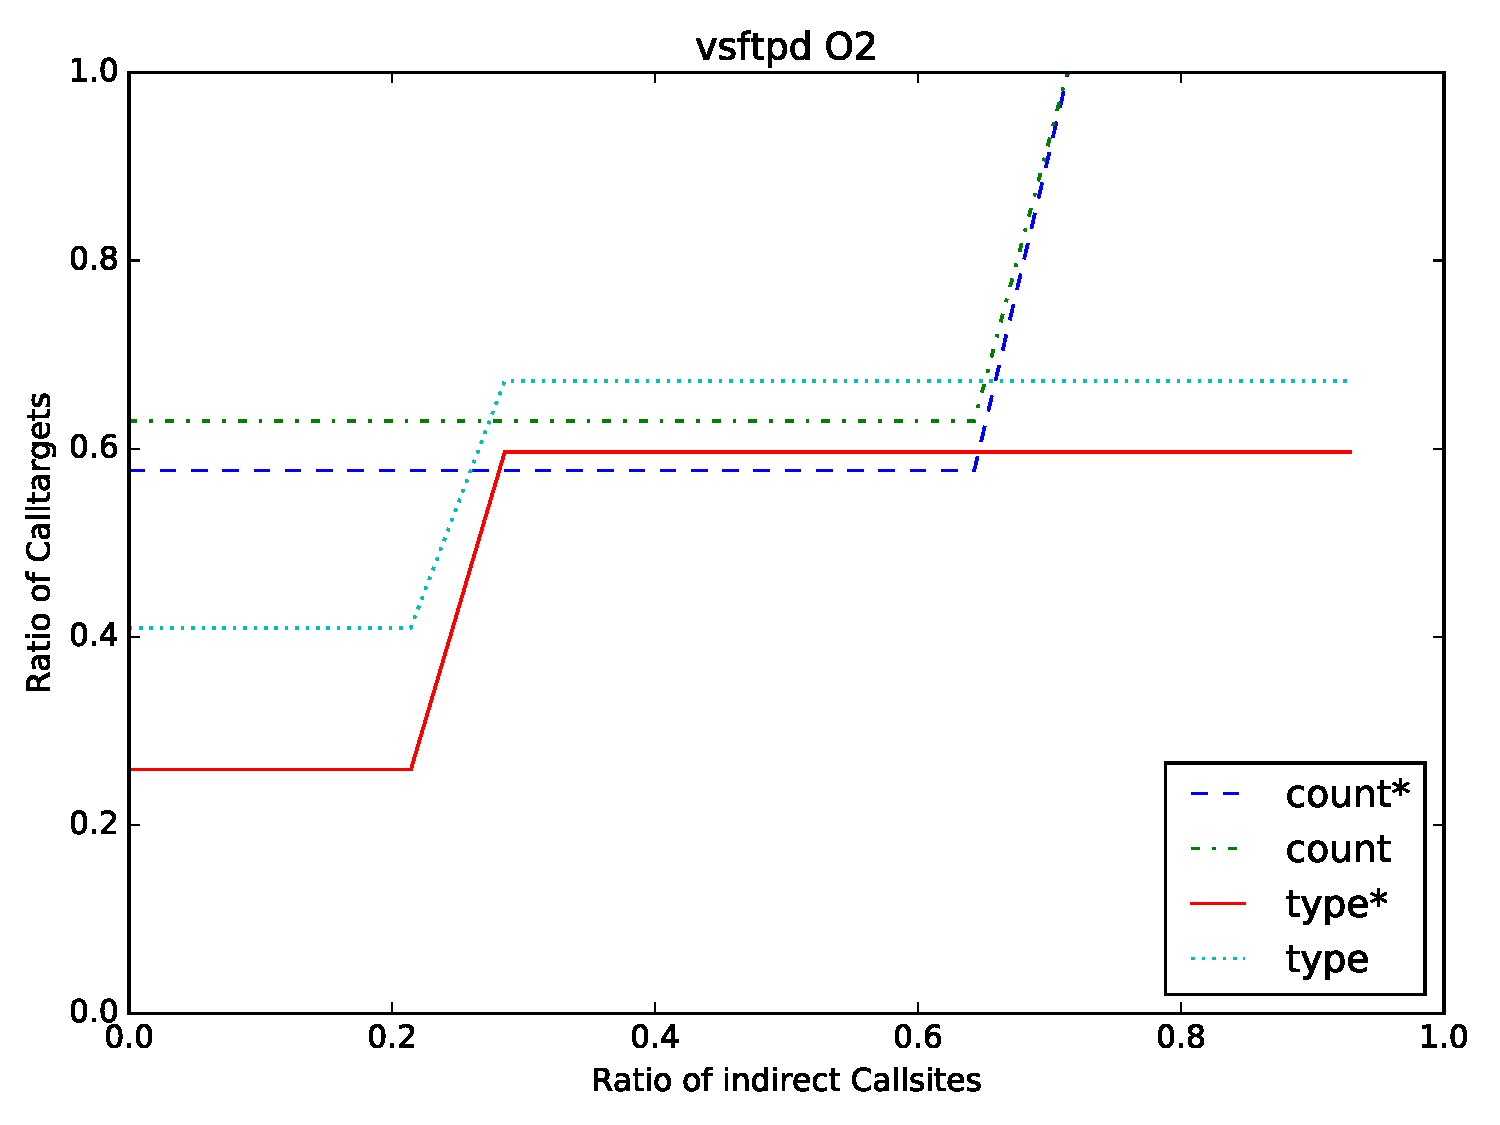
\includegraphics[width=0.5\textwidth]{../MA_Pictures/vsftpd.pdf}
%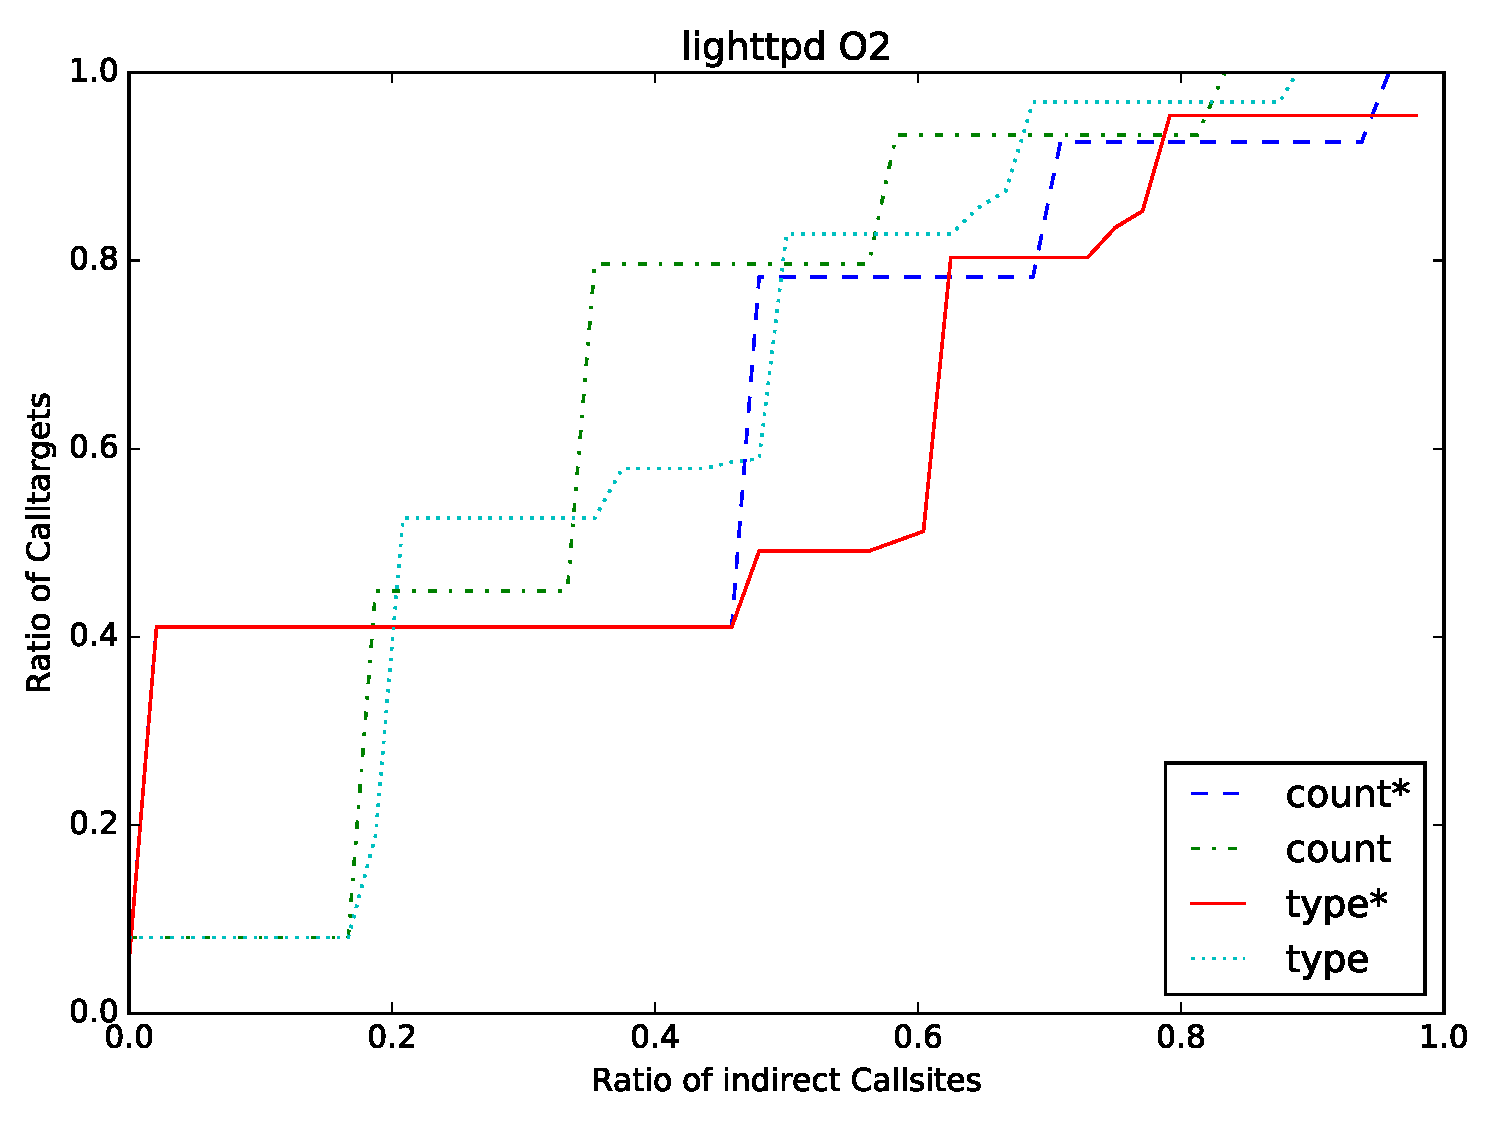
\includegraphics[width=0.5\textwidth]{../MA_Pictures/lighttpd.pdf}\\
%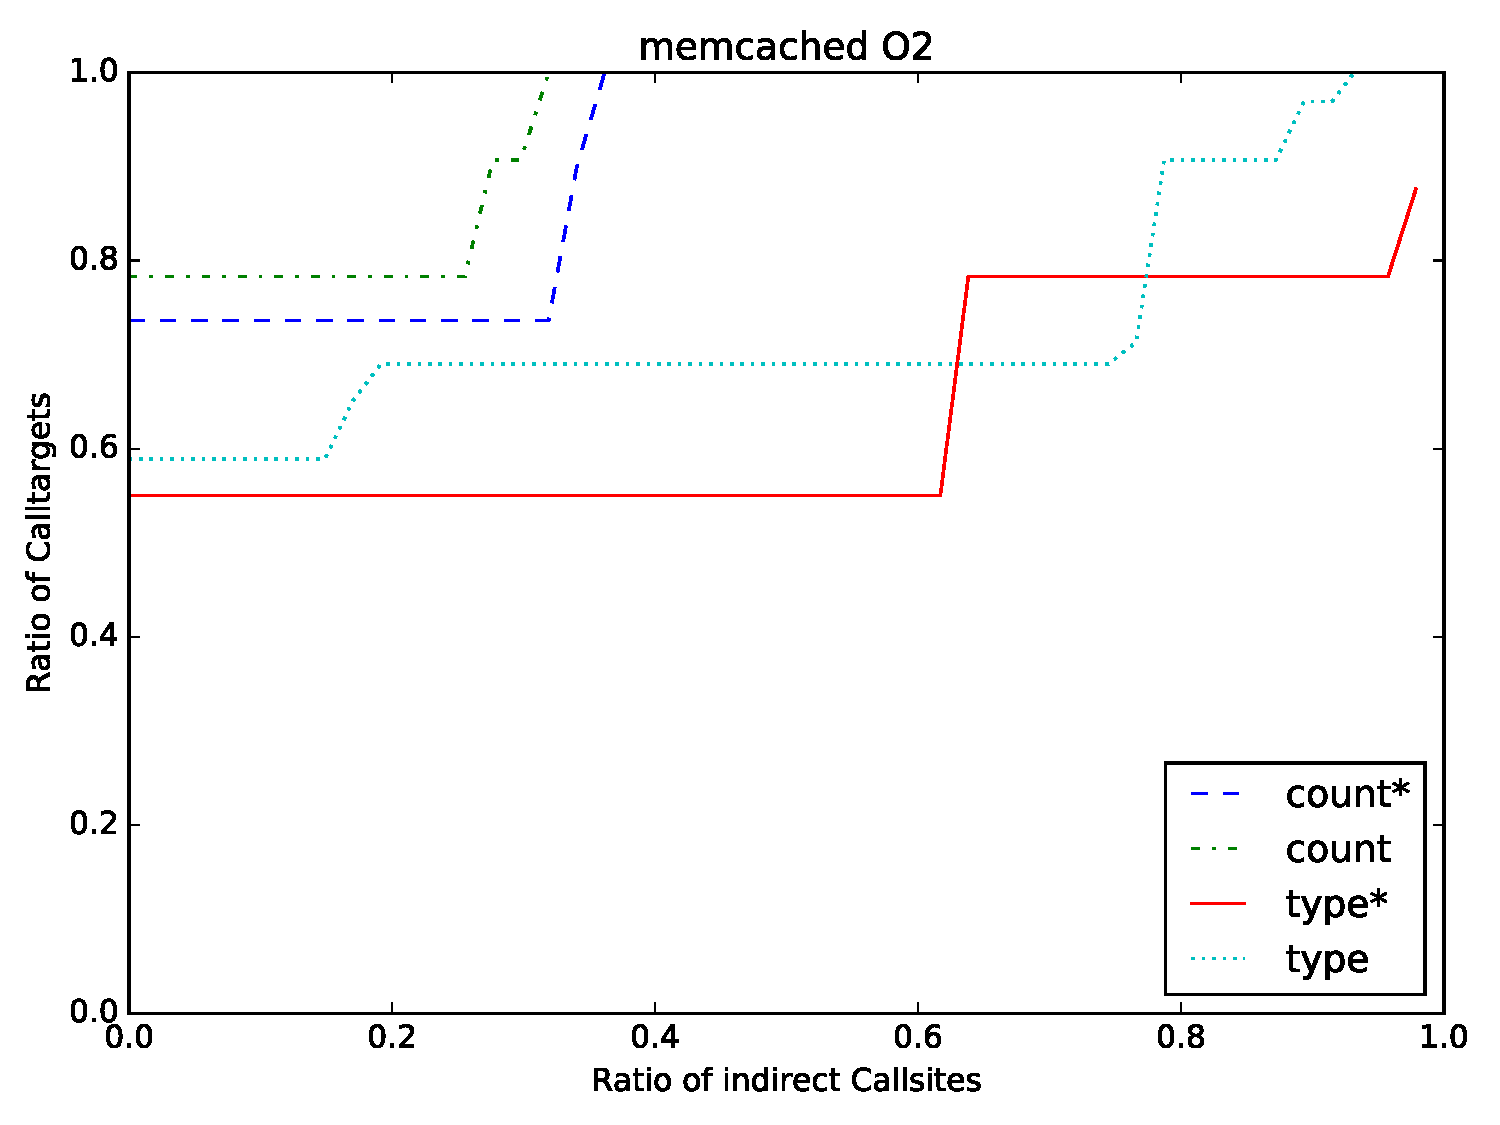
\includegraphics[width=0.5\textwidth]{../MA_Pictures/memcached.pdf}
%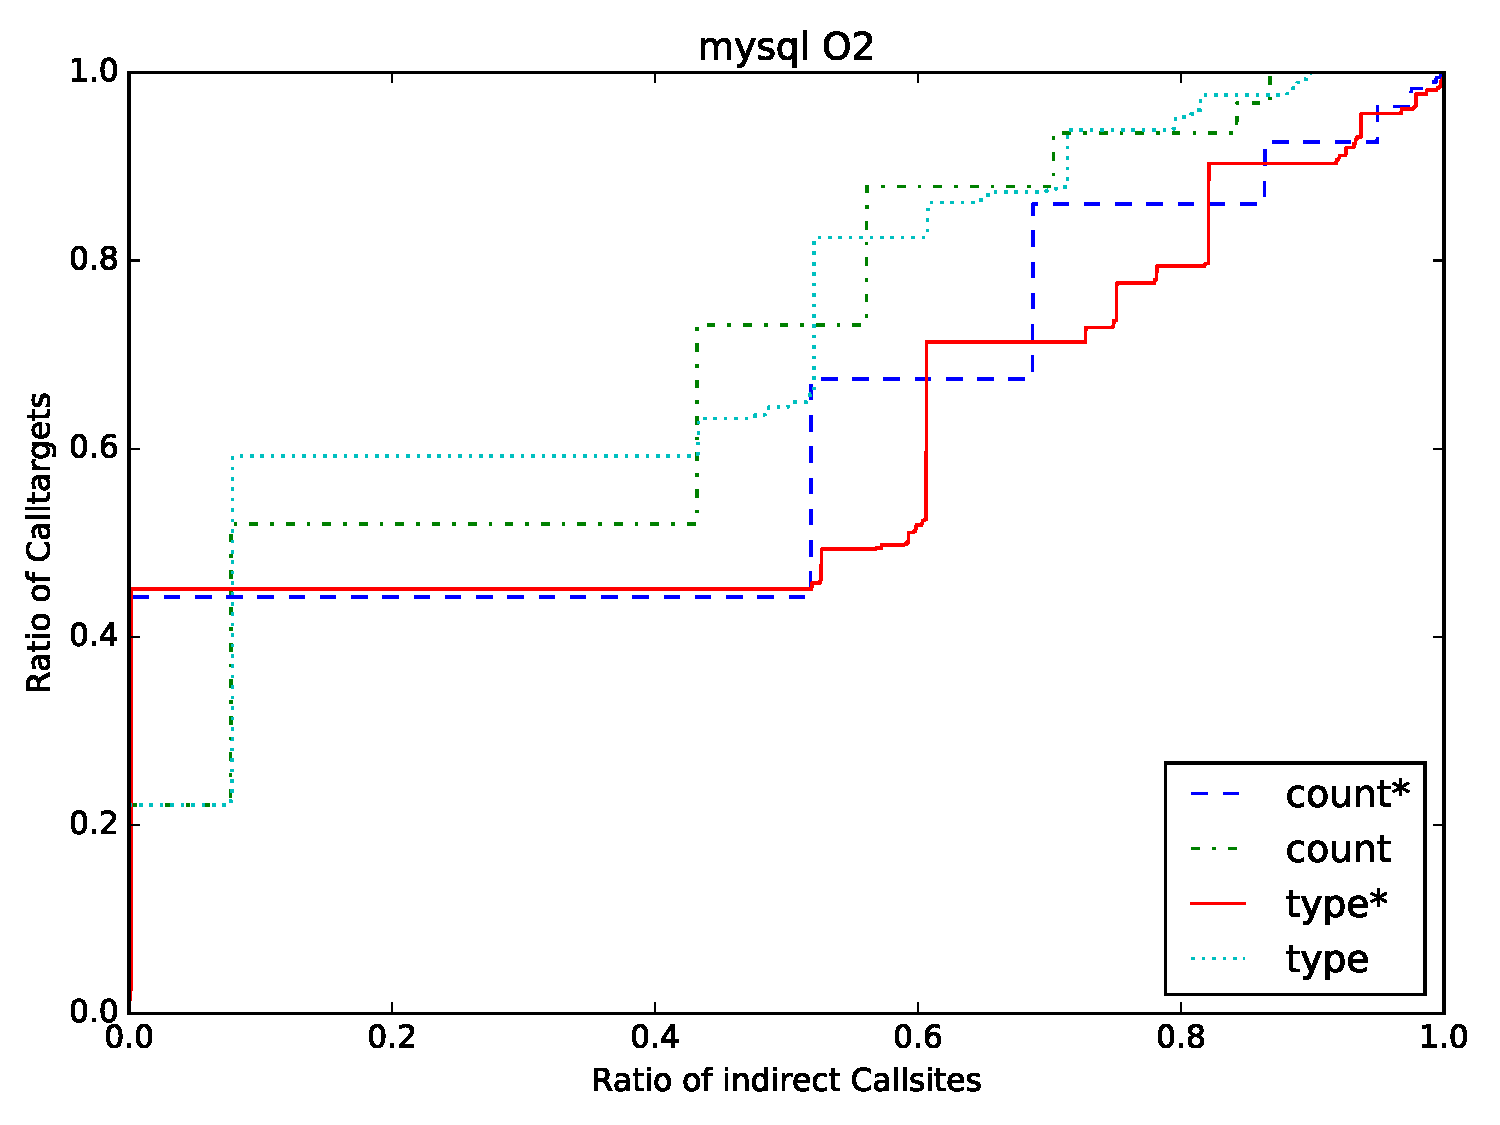
\includegraphics[width=0.5\textwidth]{../MA_Pictures/mysql.pdf}\\
%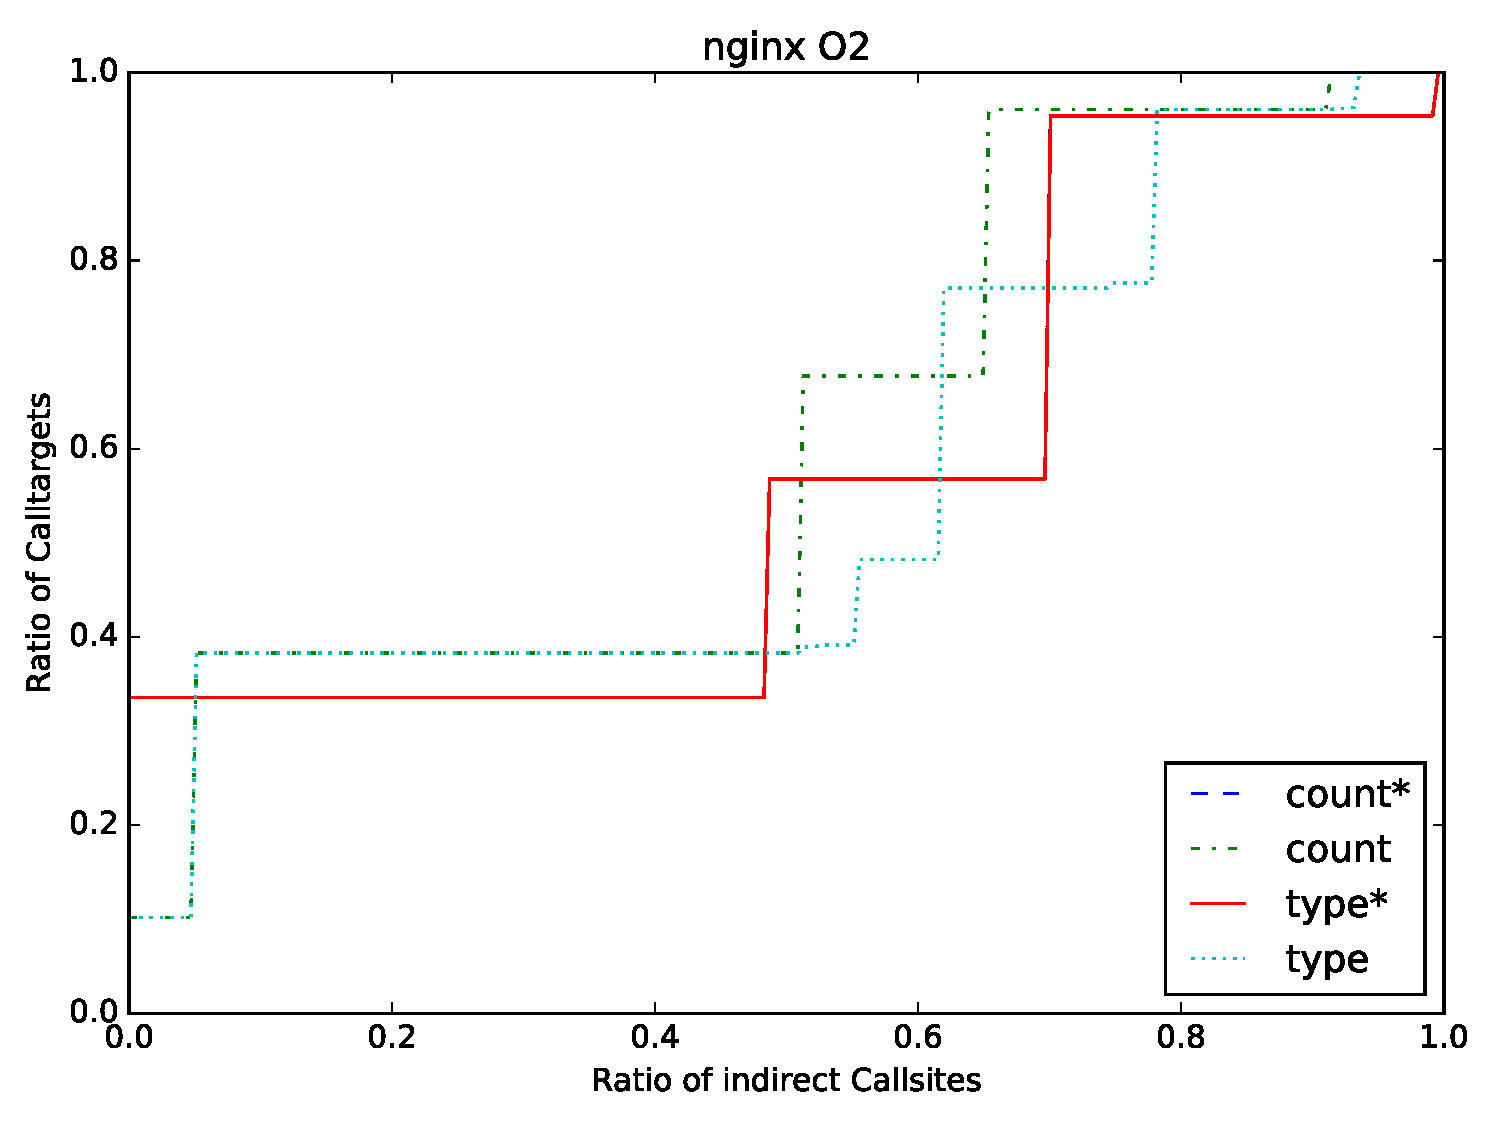
\includegraphics[width=0.5\textwidth]{../MA_Pictures/nginx.pdf}
%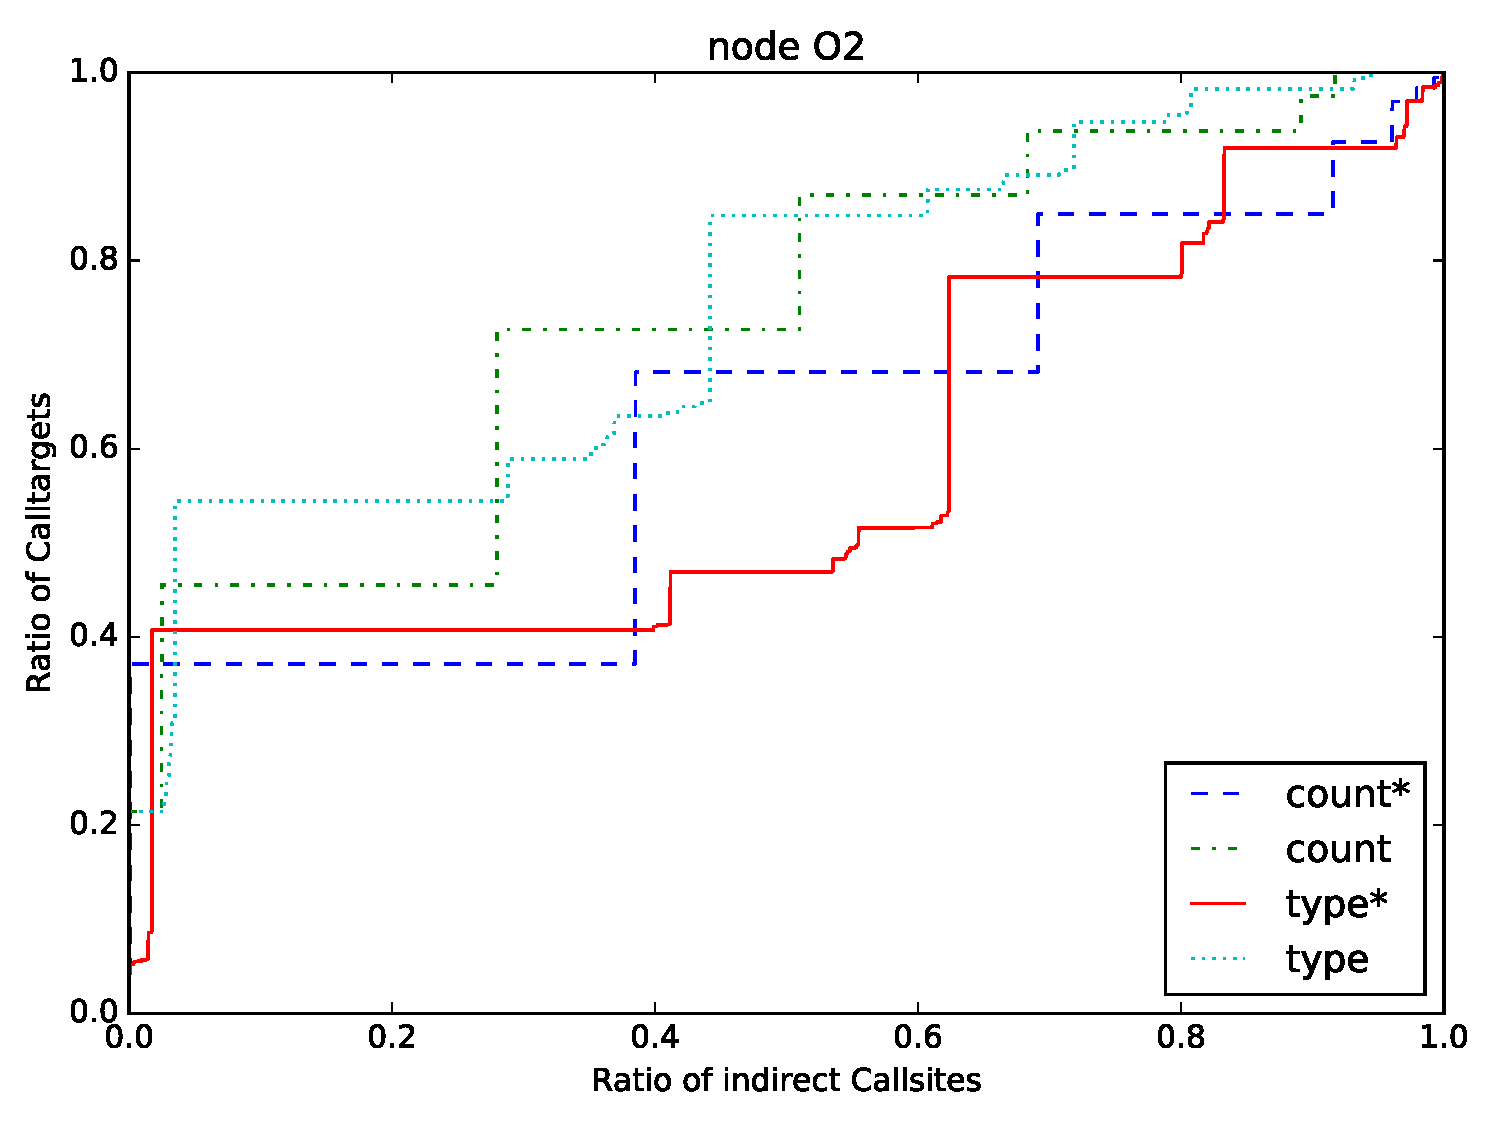
\includegraphics[width=0.5\textwidth]{../MA_Pictures/node.pdf}\\
%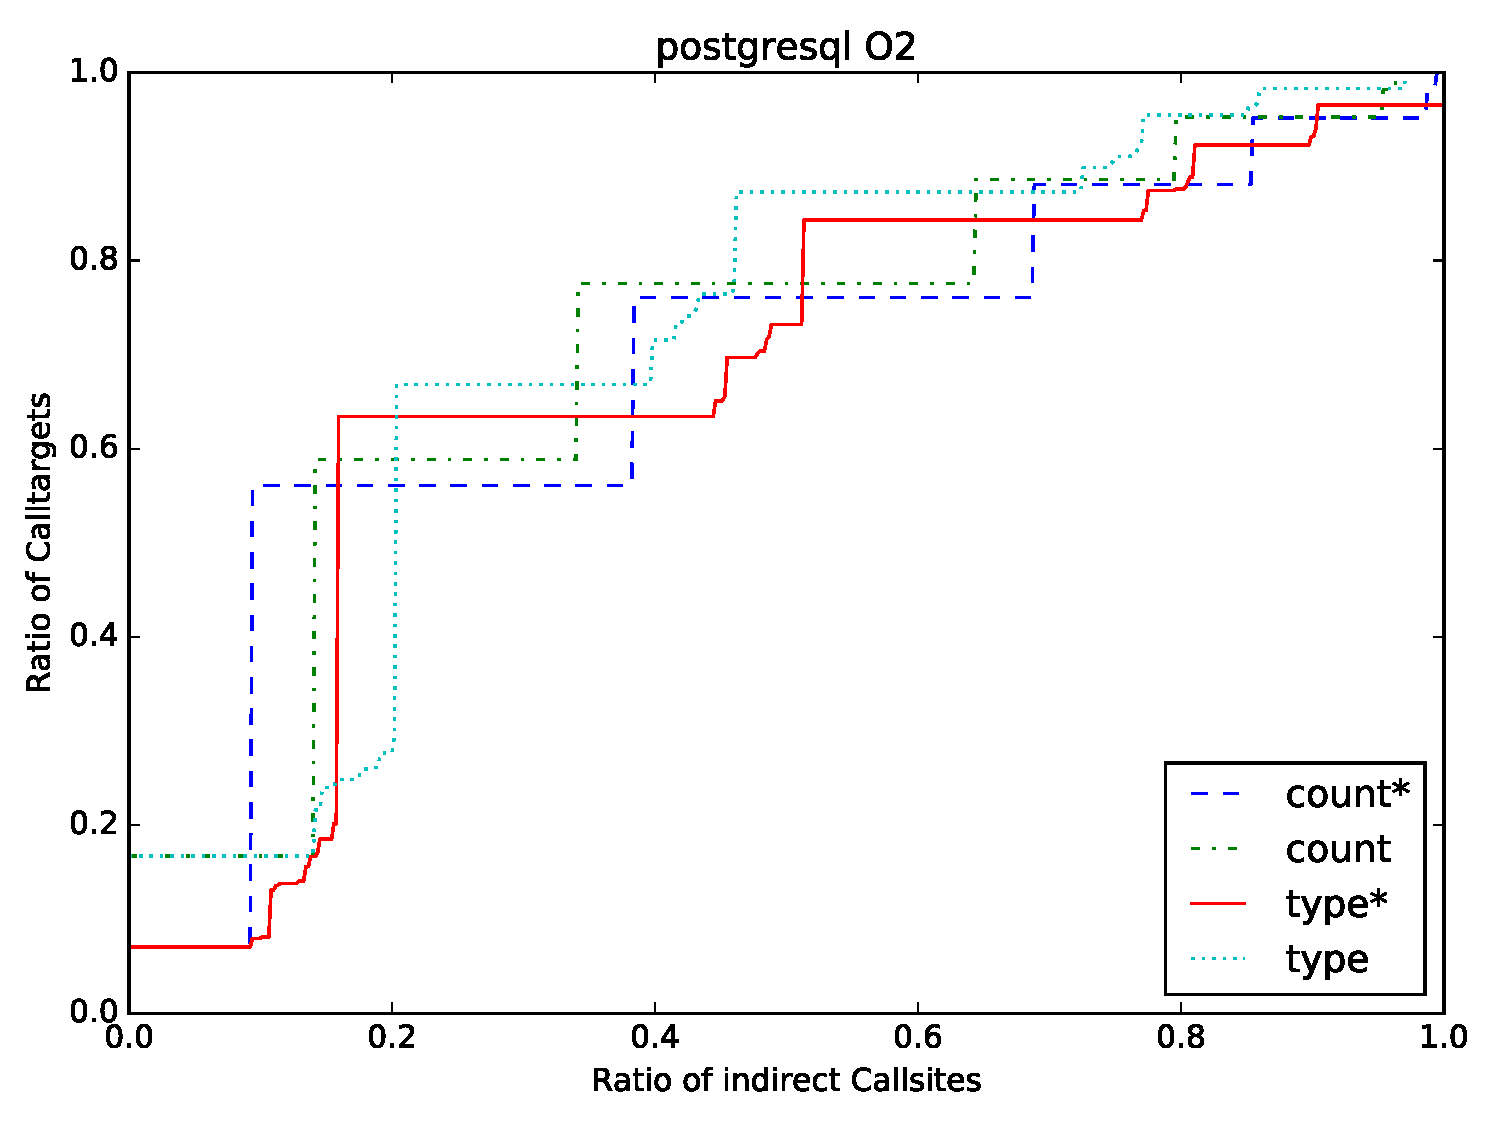
\includegraphics[width=0.5\textwidth]{../MA_Pictures/postgresql.pdf}
%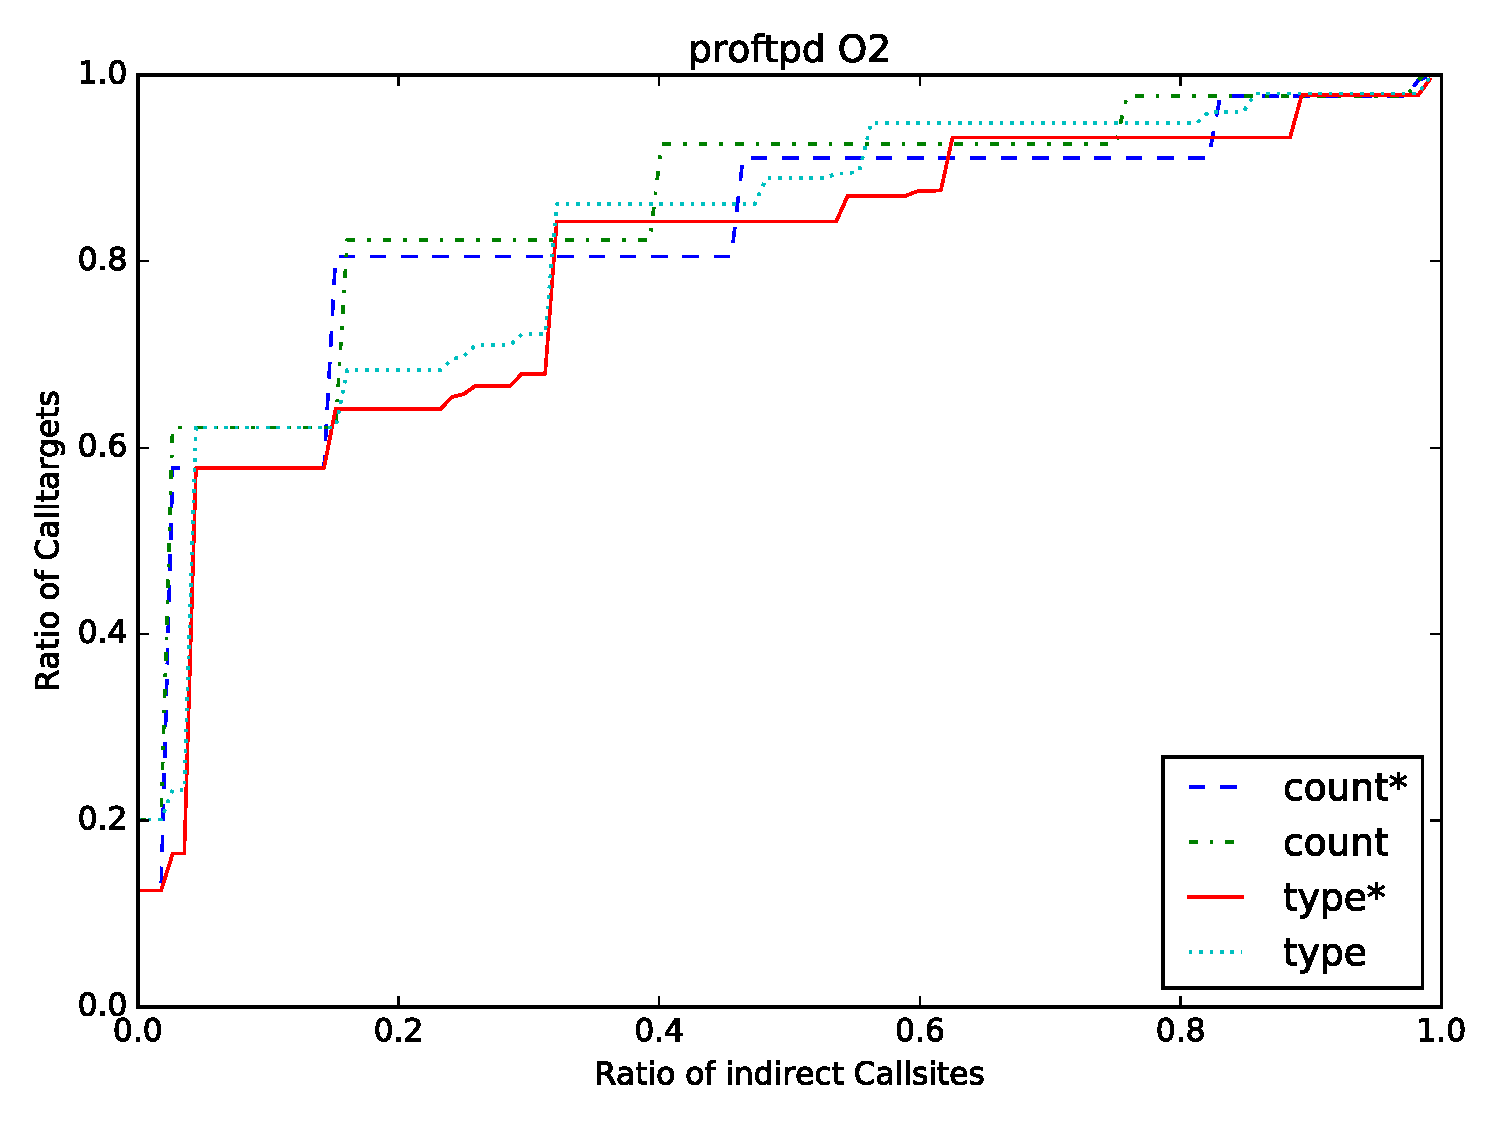
\includegraphics[width=0.5\textwidth]{../MA_Pictures/proftpd.pdf}
%\end{figure}
%

\subsubsection{CDF Analysis}
\label{CDF Analysis}

\begin{figure}[ht] 
  \label{ fig7} 
  \begin{minipage}[b]{0.5\linewidth}
    \centering
    \resizebox{1.04\columnwidth}{!}{\includesvg{postgresqlO2}}
    \caption{postgresql} 
    \vspace{4ex}
  \end{minipage}%%
  \begin{minipage}[b]{0.5\linewidth}
    \centering
    \resizebox{1.04\columnwidth}{!}{\includesvg{nodeO2}} 
    \caption{node.js} 
    \vspace{4ex}
  \end{minipage} 
  \begin{minipage}[b]{0.5\linewidth}
    \centering
    \resizebox{1.04\columnwidth}{!}{\includesvg{proftpdO2}}
    \caption{proftpd} 
    \vspace{4ex}
  \end{minipage}%% 
  \begin{minipage}[b]{0.5\linewidth}
    \centering
    \resizebox{1.04\columnwidth}{!}{\includesvg{mysqlO2}} 
    \caption{mysql} 
    \vspace{4ex}
  \end{minipage} 
\end{figure}

When looking at the CDFs of legal callsite targets as shown for postgresql \ref{fig7}, node.js \ref{fig8}, proftpd \ref{fig9}, mysql \ref{fig10}, one should instantly see the difference between the type and the count policies. While the count  policies have only a few number of changes, the number of changes that can be seen within the type policies is vastly higher. The reason for that is simple, the number of buckets that are used to classify the callsites and calltargets is simply higher. While type policies mostly perform better than the count policies, there are still parts within the type plot that are above the count plot, the reason for that is relatively simple: the maximum number of calltargets a callsite can access has been reduced, therefore a lower amount of calltargets is a higher percentage than before. However all of that is also dependent on the structure of the program.

\subsection{RQ3: Runtime Performance Overhead}
In general, we have usually about 2\%-5\% performance drop when instrumenting using Dyninst. The reason for that are essentially cachemisses introduced by jumping between the old and the new executable section of the binary generated by duplicating and patching the duplicate. This is necessary, because when out side of the compiler it is nigh on impossible to relocate indirect controlflow, therefore everytime an indirect control flow occurs, one jumps into the old executable section and from there back to the new executable section. Mroeover this is also dependent on the actual structure of the target, as it depends on the number of indirect controlflow operations per time unit.

\label{section:typeshieldoverheadperformance}
\todo[inline]{In this section we need one or two Table similar to what TypeArmor contains, first we need to define the fields which make most sense.}
\begin{figure}[htbp!]
    \centering
    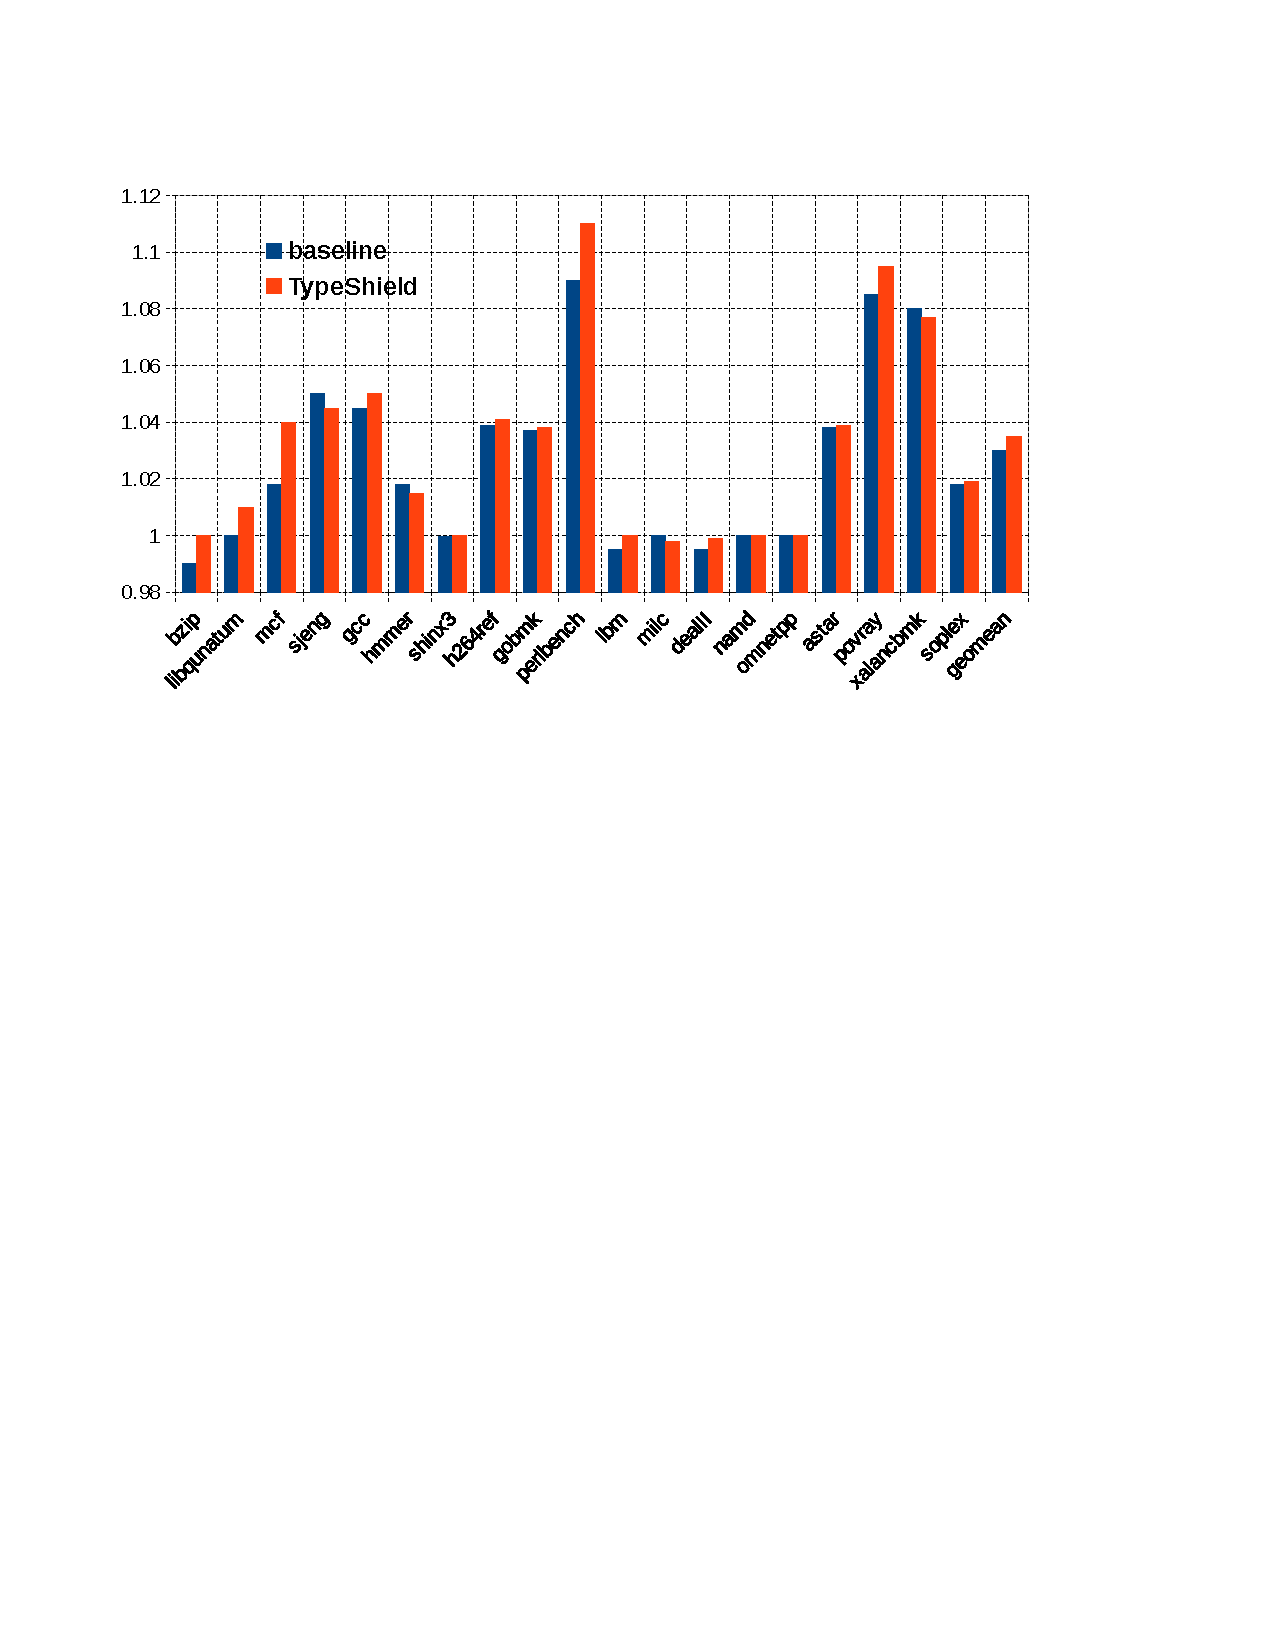
\includegraphics[width=0.49\textwidth]{figures/speccpu2006.pdf}
    \caption{Awesome Image}
    \label{fig:awesome_image}
\end{figure}
\todo[inline]{add a binary patch that does not crash none of the programs from SPEC2006.}
\todo[inline]{need a table with all the results for each of the SPEC2006 programs and a bar diagram}

\subsection{RQ4: Instrumentation Overhead}
\label{section:typeshieldoverheadinstrumentation}

\todo[inline]{here we need a bar chart, see TypeArmor paper.}
\todo[inline]{Measure the size (in bytes) of the SPEC2006 testes in RQ3 before and after adding all the patches}

The instrumentation overhead or the change in size due to patching is mostly due to the method Dyninst uses to patch binaries. 
Essentially the executable part of the binary is duplicated and extended with the patch. The usual ratio is around 40\% to 
60\% while postgres has an increase of 150\% in binary size. One cannot reduce that value significantly, 
because of the nature of code relocation after losing the data that a compiler has. Especially indirect control flow 
changes are very hard to relocate. Therefore instead each important basic block in the old code contains a jump 
instruction to the new position of the basic block.

\subsection{RQ5: Comparisons with Other Tools}
\label{RQ5: Is TypeShield better than other tools?}
\begin{table}[h!]
\resizebox{\columnwidth}{!}{
	\begin{tabular}{l|r|r|r|r|r}%
	\toprule
	\bfseries Target & AT & TypeArmor  &  IFCC &  TypeShield (count) & TypeShield (type)% specify table head
	\\\midrule
	\csvreader[before filter=\ifthenelse{\equal{\csvcolii}{geomean}}{\csvfilterreject}{\csvfilteraccept},  late after line=\\, late after last line=\\\midrule]{csvs/tools_compare.csv}{
		%1=\target, 2=\opt, 3=\fns, 4=\fnsnotClang, 5=\fnsnotpadyn, 6=\ats, 7=\atnotClang, 8=\atnotpadyn, 9=\cscount, 10=\csClang, 11=\cspadyn
	}
	{\csvcolii & \csvcoliii & \csvcoliv & \csvcolv & \csvcolvi & \csvcolvii}% specify your coloumns here

	\csvreader[before filter=\ifthenelse{\equal{\csvcolii}{geomean}}{\csvfilteraccept}{\csvfilterreject},  late after line=\\, late after last line=\\\bottomrule]{csvs/tools_compare.csv}{
		%1=\target, 2=\opt, 3=\fns, 4=\fnsnotClang, 5=\fnsnotpadyn, 6=\ats, 7=\atnotClang, 8=\atnotpadyn, 9=\cscount, 10=\csClang, 11=\cspadyn
	}
	{\csvcolii & \csvcoliii & \csvcoliv & \csvcolv & \csvcolvi & \csvcolvii}% specify your coloumns here
    	\end{tabular}}
%     	}
	\caption {The medians of calltargets per callsite for different tools that we have values for}
	\label{tbl:toolcompare}
\end{table}

Table~\ref{tbl:toolcompare} depicts a comparison between \textsc{TypeShield}, TypeArmor and IFCC w.r.t. the count of calltargets per callsites.
The values depicted in this table for TypeArmor and IFCC are taken from the original TypeArmor paper.
We compare our version of address taken analysis (AT), TypeArmor, TypeShield (count), TypeShield (type) and IFCC. 
The first thing to notice is that when comparing these values, one can see that we did not implemented a separation based on return type or the 
CFC that TypeArmour introduced. Therefore when implementing those measures, we predict that our solution would improve even more in w.r.t precision.
While we think it is possible to surpass TypeArmor implementing those two solutions in our tool, we deem it nigh on impossible to be able to compete with IFCC,
which can directly operate on the sourcecode level. Therefore it has access to more possibilities than simply inspecting the parameters or return values.






		\section{Related Work}
\label{chapter:Related_Work}

\textbf{Type-Inference on Executables.}
\label{Type-Inference on Executables}
Recovering variable types from executable programs
is very hard in general for several reasons. 
First, the quality of the disasembly can very much from used
framework to another. \textsc{TypeShield} is based on DynInst 
and the quality of the execuatble disasembly fits our needs. 
For a more comprehensive review on the capabilities of DynInst and other tools we
advice the reader to have a look at~\cite{andriesse:indepth}.
Second, alias analysis in binares is undecidable in theory and intractable in practice~\cite{alan:mycroft}.
There are several most promising tools such as: Rewards~\cite{lin:rewards}, BAP~\cite{bap:brumley}, 
SmartDec~\cite{fokin:smartdec}, and Divine~\cite{divine:balakrishnan}.
These tools try with more or less success to recover 
type information from binary programs with different goals.
Typical goals are: 
\textit{i)} full program reconstruction (binary to code convertion, reversing), 
\textit{ii)} checking for buffer overflows, 
\textit{iii)} integer overflows and other types of memory corruptions.
For a more exhaustive review of such tools we advice the reader to
have a look at the review of Caballero et al.~\cite{caballero:inference}.
Intresting to notice is that the code from only a few of this tools is available.

While smartde seemed promising due to its simple type lattice that we wanted to leverage for our classification schema. Its integration into our DynInst based environment was not successful mostly for time constraints, as it was deemed to time consuming to extract the whole machinery and implemnt an interface to the DynInst disassembler.
Therefore we finally implemented our own version of type analysis and only focused on the wideness of the types, resulting in a simpler lattice than we initially wanted.

%maybe not relevant
\textbf{Mitigation of Code-Reuse Attacks.}
\label{Mitigation of Code-Reuse Attacks}
In the last couple of years researchers have provided many versions of new Code Reuse Attacks (CRAs).
These new attacks were possible since DEP~\cite{dep} and ASLR~\cite{ASLR} were successfully bypassed mostly based
on Return Oriented Programming (ROP)~\cite{ROP, kornau:rop, rop:shacham} on one hand and on 
the other hand due to the discovery of new exploitable hardware and software primitives.

ROP started to present itself in the last couple of years in many faceted ways such as:
Jump Oriented Programming (JOP)~\cite{JOP1, JOP2, JOP3} which uses jumps in order to divert the control flow to the next gadget and 
Call Oriented Programming (COP)~\cite{rop:carlini} which uses calls in order to chain gadgets together.
CRAs have many manifestations and it is out of scope of this work to list them all.

On one hand, CRAs can be mitigated in general in the following ways: 
\textit{(i)} binary instrumentation,
\textit{(ii)} source code recompilation and 
\textit{(iii)} runtime application monitoring.
On the other hand, there is a plethora of tools and techniques which try to enforce CFI based
primitives in executables, source code and during runtime. Next we briefly
present the solution landscape together with the approaches and the techniques on which these are based:
\textit{(a)} fine-grained CFI with hardware support, PathArmor~\cite{veen:cfi},
\textit((b)) coarse-grained CFI used for binary instrumentation, CCFIR~\cite{ccfir:zhang},
\textit{(c)} coarse-grained CFI based on binary loader, CFCI~\cite{cfci:zhang}
\textit{(d)} fine-grained code randomization, O-CFI~\cite{mohan:opaque},
\textit{(e)} cryptografy with hardware support, CCFI~\cite{ccfi:jose},
\textit{(f)} ROP stack pivoting, PBlocker~\cite{pblocker:prakash},
\textit{(g)} canary based protection, DynaGuard~\cite{dynaguard:petsios},
\textit{(h)} runtime and hardware support based on a combination of LBR, PMU and BTS registers CFIGuard~\cite{cfiguard:yuan}, and
\textit{(i)} source code recompilation with CFI and/or randomization enforcement against JIT-ROP attacks, MCFI~\cite{mcfi:niu}, 
RockJIT~\cite{rockjit:niu} and PiCFI~\cite{perinput:niu}.

The above list is not exhaustive and new protection techniques can be obtained by combining available techniques
or by using newly available hardware features or software exploits. However, none of the above techniques and tools 
can mitigate against COOP attacks.


% \textbf{Mitigation of Advanced Code-Reuse Attacks.}
\textbf{Mitigation of Forward-Edge based Attacks.}
\label{Mitigation of Advanced Code-Reuse Attacks}
Recur-sive-COOP~\cite{crane:readactor++}, COOP~\cite{schuster:coop} and Subversive-C~\cite{subversive-c:lettner}.
are advanced CRAs since these attacks can not be addressed:
\textit{i)}  with shadow stacks techniques (i.e., do not violate the caller/calle convention), 
\textit{ii)} coarse-grained Control-Flow Integrity (CFI)~\cite{abadi:cfi2, abadi:cfi} techniques are useless against these attacks, 
\textit{iii)} hardware based approaches such as Intel CET~\cite{intel:cet} can not mitigate this attack for the same reason as in \textit{i)}, and 
\textit{iv)} with OS-based approaches such as Windows Control Flow Guard~\cite{windows:cfguard} 
since the precomputed CFG does not contain edges for indirect call sites which are explicitly exploited during the COOP attack.
However, the following tools can protect against COOP attacks:

\textit{Source code based.} Indirect call site targets are checked based on vTable integrity.
Different types of CFI policies are used such as in the following tools:
SafeDispatch~\cite{safedispatch:jang}, IFCC/VTV~\cite{vtv:tice} LLVM and GCC compiler.
Additionally, the Redactor++~\cite{crane:readactor++} uses randomization 
vTrust~\cite{zhang:vtrust} checks call target function signatures, 
CPI~\cite{volodymyr:cpi} uses a memory safety technique
in order to protect against the COOP attack.

There are several source code based tools 
which can successfully protect against the COOP attack.
Such tools are: ShrinkWrap~\cite{haller:shrinkwrap}, IFCC/VTV~\cite{vtv:tice}, 
SafeDispatch~\cite{safedispatch:jang}, vTrust~\cite{zhang:vtrust}, Readactor++~\cite{crane:readactor++}, CPI~\cite{volodymyr:cpi} and the
tool presented by Bounov et al.~\cite{bounov:interleaving}. These tools profit from high precision
since they have access to the full semantic context of the program though the scope
of the compiler on which they are based. 
Because of this reason these tools target mostly other types of security problems than binary-based 
tools address. For example some last advancec in compile based protection against 
code reuse attacks address mainly performance issues.
Currently, most of the above presented tools are only forward
edge enforcers of fine-grained CFI policies with an overhead from 1\% up to 15\%.

We are aware that there is still a long research path to go until binary based techniques can 
recuperate program based semantic information from executable with the same precision as compiler based tools.
These path could be even endless since compilers are optimized for speed and are designed to remove as much as possbile semantic information
from an executable in order to make the program run as fast as possible. In light of this fact,
\textsc{TypeShield} is another attempt to recuperate just the needed semantic information (types and number of function parameters from
indirect call sites) in order to be able to enforce a precise and with low overhead primitive against COOP attacks.

Rather than claiming that the invariants offered by \textsc{TypeShield} are suffiecient
to mitigate all versions of the COOP attack we take a more conservative path by claiming that \textsc{TypeShield} 
further raises the bar w.r.t. what is possible when defending against COOP attacks on the binary level.

\textit{Binary based.} vTable protection is addressed through binary instrumentation in tools
such as: vfGuard~\cite{vfuard:aravind}, vTint~\cite{vtint:zhang}. However, none of these tools can
help to mitigate against COOP. The only binary based tool which we are aware of that
can mitigate protect against COOP is TypeArmor~\cite{veen:typearmor}.  
TypeArmor uses a fine-grained CFI policy based on caller (only indirect call sites)/callee matching 
which consists in checking during runtime if the number of provided and needed parameters match.

\textsc{TypeShield} is most similar to TypeArmor~\cite{veen:typearmor} since
we also enforce strong binary-level invariants on the number of function
paramters. \textsc{TypeShield} similarly to TypeArmor targets 
exclusive protection against advanced exploitation techniques 
which can bypass fine-grained CFI schemes and VTable protections at the binary level.

However, \textsc{TypeShield} offers a better restriction of call targets to call sites, since 
we not only restrict based on the number of parameters but also on the wideness of their types. 
This results in much smaller buckets that in turn can only target a smaller subset of all address
taken functions. However, we rely for that on the variety of parameter types and when there is 
none, we will degrade into a parameter count policy.

\textit{Runtime based.}
``There is something available out there but I can not use it'' \textit{Anonymous}.
Long story short conclusion: There are several promising runtime-based line of defenses against
advanced CRAs but none of them can successfully protect against the COOP attack.

IntelCET~\cite{intel:cet} is based on, \texttt{ENDBRANCH}, a new CPU instruction which can be used to enforce
an efficient shadow stack mechanism. The shadow stack can be used to check during program execution if caller/return pairs match.
Since the COOP attack reuses whole functions as gadgets and does not violate the caller/return convention than the 
new feature provided by intel is useless in the face of this attack. Nevertheless other highly notorious CRAs may not be possible
after this feature will be implemented main stream in OSs and compilers.

Windows Control Flow Guard~\cite{windows:cfguard} is based on a user-space and kernel-space components which
by working closely together can enforce an efficient fine-grained CFI policy based on a precomputed CFG.
These new feature available in Windows 10 can considerably rise the bar for future attacks but in our opinion advanced CRAs
such as COOP are still possible due the typical characteristics of COOP.

PathArmor~\cite{veen:cfi} is yet another tool which is based on a precomputed CFG and on the LBR register which can give a string of 16 up to
32 pairs of from/to addressed of different types of indirect instructions such as \texttt{call}, \texttt{ret}, and \texttt{jump}. 
Because of the sporadic query of the LBR register (only during invocation of certain function calls) and because of the sheer amount of 
data which passes through the LBR register this approach has in our opinion a fair potential to catch different types of CRAs but
we think that against COOP this tool can not be used. First, because of the fact that the precomputed CFG does not contain edges for all
possible indirect call sites which are accessed during runtime and second, the LBR buffer can be easily triked by adding
legitimate indirect call sites  during the COOP attack.


		\section{Discussion}
\label{chapter:Discussion}

\textbf{Comparison with TypeArmor.}
\label{section:comptype}
We are looking at two sets of results. First of all, we compare the overall precision of our implementation
of the COUNT policy with the results from TypeArmor to set the perspective for the precision of our TYPE 
policy. We cannot compare data regarding overestimations of calltargets or underestimations of callsites, 
as TypeArmor did not provide sufficient data. The second point of comparison is the reduction of calltargets
per callsite, however, this comparison is rather crude, as we most surely do not have the same measuring
environment and not sufficient data to infer its quality.

\textit{Precision of Classification.}
TypeArmor reports a geometric mean of 83.26\% for the perfect classification of calltargets regarding 
parameter count in optimization level O2, which compares rather well to our result of 82.24\%. Regarding
the perfect classification of callsites we report a geometric mean of 81.6\% perfect classification 
regarding parameter count, while TypeArmor reprots a geometric mean of 79.19\%. Howevver we also have
a geometric mean of about 7\% regarding underestimations in the callsite classification with an upper
bound of 16\%, while TypeArmor reports that it does not incur underestimations in their callsites.
Now, for our type based classification we incur the cost for two error sources. First, the error from
the parameter count classification, which we base our type analysis on and second for the type analysis
itself. The numbers for the perfect classification of calltargets regarding parameter types we report a
72.25\% geometric mean of perfect classification, which is 87.85\% of our precision regarding parameter
counts. However we report a geometric mean of 57.36\%
for perfect classification of callsites, which altough seemingly low, is still 69.74\% of our precsion
regarding parameter counts.

\textit{Reduction of Available Calltargets}
While our count based precision focused implementation achieves a reduction in the same ballpark as
TypeArmour regarding our test targets, lets us believe that our implementation of their classification
schema is a sufficient approximation to compare against. However, we cannot safely compare those numbers,
as the information regarding their test environment are rather sparse and the only data available is the
median, which in our opinion does discard valuable information from the actual result set. This is the
main reason we implemented an approximation, because we needed more metrics to compare \textsc{TypeShield}
and TypeArmor regarding calltargets. Using average and sigma, we can report that our precision focused
type based classification can reduce the number of calltargets, by up to 20\% more than parameter number
based classification with an overall reduction of about 9\%.


\textbf{TypeArmor Discrepancies.}
\label{section:discrep}
As we have no access to source code of TypeArmor, we habe implemented an approximation
of TypeArmor. Using this approximation we found some discrepancies between the data that we collected
and data that was presented.
A minor discrepancy between our results and the results of TypeArmor is that, while they basically implemented
what we call a destructive merge operator for the liveness analysis. However, our data suggestes that this
operator is marginally inferior to the union pathmerge operator, when we compared them in our implementation.
A major concern is the classification of calltargets, while we were able to reduce the number of overerstimations
of calltargets regarding parameter counts to essentially 0, the number of underestimations of calltarget did
stay at a geometric mean of 7\%. This error rate is rather large when compared to the reported 0\% underestimation
of TypeArmor, however we are not entirely sure what has caused this discrepancy. A possibility is the differing
test environments, or a bug within our implementation that we are not aware of, or simply reaching defintions
analysis alone is not the best possible algorithm for this particular problem.

\textbf{Improving \textsc{TypeShield}.}
\label{section:venuesimp}
To improve our type analysis, we see atleast two possibilities. Incorporating refined dataflow analysis and 
expanding the scope to also include memory. The main point of improvement is not the precision but for now 
more importantly the reduction of underestimations in the callsite analysis.

To refine the dataflow analysis, we propse the actual tracking of data values and simple operations, as these
can be used to better differentiate the actual wideness stored within the current register. The highest gain, 
we see here would be the establishment of upper and lower bounds regarding values within the register, which 
would allow for more sophisticated callsite and calltarget invariants. Essentially we would have to resort 
to symbolic execution or some other sort of precise abstract interpretation.

Expanding the scope to also include memory, is another possible way of improving the type analysis, as it 
would allow us to distinguish normal 32 or 64 bit values and pointer addresses. Although we already have a 
limited approach of that in our reaching implementation, we still see room for improvement, as we only check
whether a value is within one of three binary sections or 0.

\textbf{Limitations of \textsc{TypeShield}.}
\label{section:limit}
First of all, we are limited by the capabilities of the DynInst Instrumentation Environment, the main problem,
we are facing here is that non returning functions like exit are not detected reliably in some cases, which is
why we were not able to test the Pure-FTP server, as it heavily relies on these functions. The problem is that
those non returning functions usually appear as a second branch within a function that occurs after the normal
control flow, causing basic blocks from the following function to be attributed to the current function. This
results in a malformed control flow graph and erroneous attribution of callsites and problematic misclassifications
for both calltargets and callsites.

Another limitation of \textsc{TypeShield} is it reliance on variety within the binary, in particular we rely on
the fact that functions use more than only 64bit values or pointers within their parameter list. Should this
scenario occur, our analysis has nothing to work with and essentially degrades into a parameter count based
implementation. Thankfully this occurrence is quite rare, as we experienced within our experiments. When working
based on source level information, we could not detect a difference between our TYPE and a COUNT policies. 
However when leveraging our tool, we were able to detect differences, which reinforces the fact, that we do 
not rely on declaration of parameters but usage of those.

		\chapter{Conclusion and Future Work}
\label{chapter:Conclusion_and_Future_Work}
This section should be no longer than 2 pages. idealy exactly 2 pages would be sufficient.

\section{Conclusion} 
In this research, we presented our tool X, .... \\

Specify the points you want to talk about. Write 2-3 sentences about each point. \\

\textbf{Point 1}

\textbf{Point 2}

\textbf{Point 3}

\section{Future Work} 

In future we bla.

\textbf{Point 1}

\textbf{Point 2}

\textbf{Point 3}

Specify the points you want to talk about. Write 2-3 sentences about each point. \\
		
		
		%
		%% ---------------------------------------------------------------------------
		%%
		%% Fully Automated Calibration for Ultrasound
		%%
		%%% ---------------------------------------------------------------------------
		%\part[The 2nd Part]{The Second Part}
		%\label{part:secondP}
		
		
		% ---------------------------------------------------------------------------
		%
		% Appendix
		%
		% ---------------------------------------------------------------------------
		
		%\part*{Appendix}
		%\addcontentsline{toc}{part}{Appendix}
		
		%\appendix %---------------------------------------
		
		%\chapter{Detailed Descriptions}
%\section{Detailed Validation Results}
\label{chapter:DetailedDescriptions}
Here come the details that are not supposed to be in the regular text.
		
	


  \clearemptydoublepage
  
	\bibliography{bibliography/literature}
	
 
\end{document}

